\documentclass[a4paper]{book}
\usepackage{makeidx}
\usepackage{graphicx}
\usepackage{multicol}
\usepackage{float}
\usepackage{listings}
\usepackage{color}
\usepackage{ifthen}
\usepackage[table]{xcolor}
\usepackage{textcomp}
\usepackage{alltt}
\usepackage{ifpdf}
\ifpdf
\usepackage[pdftex,
            pagebackref=true,
            colorlinks=true,
            linkcolor=blue,
            unicode
           ]{hyperref}
\else
\usepackage[ps2pdf,
            pagebackref=true,
            colorlinks=true,
            linkcolor=blue,
            unicode
           ]{hyperref}
\usepackage{pspicture}
\fi
\usepackage[utf8]{inputenc}
\usepackage{mathptmx}
\usepackage[scaled=.90]{helvet}
\usepackage{courier}
\usepackage{doxygen}
\lstset{language=C++,inputencoding=utf8,basicstyle=\footnotesize,breaklines=true,breakatwhitespace=true,tabsize=4,numbers=left }
\makeindex
\setcounter{tocdepth}{3}
\renewcommand{\footrulewidth}{0.4pt}
\begin{document}
\hypersetup{pageanchor=false}
\begin{titlepage}
\vspace*{7cm}
\begin{center}
{\Large GOGrapher \\[1ex]\large 2.0 }\\
\vspace*{1cm}
{\large Generated by Doxygen 1.7.3}\\
\vspace*{0.5cm}
{\small Tue Mar 22 2011 13:51:23}\\
\end{center}
\end{titlepage}
\clearemptydoublepage
\pagenumbering{roman}
\tableofcontents
\clearemptydoublepage
\pagenumbering{arabic}
\hypersetup{pageanchor=true}
\chapter{Namespace Index}
\section{Packages}
Here are the packages with brief descriptions (if available):\begin{DoxyCompactList}
\item\contentsline{section}{\hyperlink{namespace_g_o_gene_graph}{GOGeneGraph} }{\pageref{namespace_g_o_gene_graph}}{}
\item\contentsline{section}{\hyperlink{namespace_g_o_gene_pubmed_graph}{GOGenePubmedGraph} }{\pageref{namespace_g_o_gene_pubmed_graph}}{}
\item\contentsline{section}{\hyperlink{namespace_g_o_graph}{GOGraph} }{\pageref{namespace_g_o_graph}}{}
\item\contentsline{section}{\hyperlink{namespace_g_o_node}{GONode} }{\pageref{namespace_g_o_node}}{}
\item\contentsline{section}{\hyperlink{namespace_g_o_obo_xml_handler}{GOOboXmlHandler} }{\pageref{namespace_g_o_obo_xml_handler}}{}
\item\contentsline{section}{\hyperlink{namespace_g_o_pubmed_graph}{GOPubmedGraph} }{\pageref{namespace_g_o_pubmed_graph}}{}
\item\contentsline{section}{\hyperlink{namespacetest}{test} }{\pageref{namespacetest}}{}
\end{DoxyCompactList}

\chapter{Class Index}
\section{Class List}
Here are the classes, structs, unions and interfaces with brief descriptions:\begin{DoxyCompactList}
\item\contentsline{section}{\hyperlink{classgographer_1_1_corpus_1_1_corpus}{gographer.Corpus.Corpus} (A collection of \hyperlink{namespacegographer_1_1_document}{Document} objects )}{\pageref{classgographer_1_1_corpus_1_1_corpus}}{}
\item\contentsline{section}{\hyperlink{classgographer_1_1_document_1_1_document}{gographer.Document.Document} (A Python object representation of a PubMed record )}{\pageref{classgographer_1_1_document_1_1_document}}{}
\item\contentsline{section}{\hyperlink{classgographer_1_1_g_o_gene_graph_1_1_g_o_gene_graph}{gographer.GOGeneGraph.GOGeneGraph} }{\pageref{classgographer_1_1_g_o_gene_graph_1_1_g_o_gene_graph}}{}
\item\contentsline{section}{\hyperlink{classgographer_1_1_g_o_gene_pubmed_graph_1_1_g_o_gene_pubmed_graph}{gographer.GOGenePubmedGraph.GOGenePubmedGraph} }{\pageref{classgographer_1_1_g_o_gene_pubmed_graph_1_1_g_o_gene_pubmed_graph}}{}
\item\contentsline{section}{\hyperlink{classgographer_1_1_g_o_graph_1_1_g_o_graph}{gographer.GOGraph.GOGraph} }{\pageref{classgographer_1_1_g_o_graph_1_1_g_o_graph}}{}
\item\contentsline{section}{\hyperlink{classgographer_1_1_g_o_node_1_1_g_o_node}{gographer.GONode.GONode} }{\pageref{classgographer_1_1_g_o_node_1_1_g_o_node}}{}
\item\contentsline{section}{\hyperlink{classgographer_1_1_g_o_obo_xml_handler_1_1_g_o_obo_xml_handler}{gographer.GOOboXmlHandler.GOOboXmlHandler} }{\pageref{classgographer_1_1_g_o_obo_xml_handler_1_1_g_o_obo_xml_handler}}{}
\item\contentsline{section}{\hyperlink{classgographer_1_1_g_o_pubmed_graph_1_1_g_o_pubmed_graph}{gographer.GOPubmedGraph.GOPubmedGraph} }{\pageref{classgographer_1_1_g_o_pubmed_graph_1_1_g_o_pubmed_graph}}{}
\item\contentsline{section}{\hyperlink{classgographer_1_1_porter_stemmer_1_1_porter_stemmer}{gographer.PorterStemmer.PorterStemmer} }{\pageref{classgographer_1_1_porter_stemmer_1_1_porter_stemmer}}{}
\item\contentsline{section}{\hyperlink{classgographer_1_1_tokenizer_1_1_tokenizer}{gographer.Tokenizer.Tokenizer} }{\pageref{classgographer_1_1_tokenizer_1_1_tokenizer}}{}
\end{DoxyCompactList}

\chapter{File Index}
\section{File List}
Here is a list of all files with brief descriptions:\begin{DoxyCompactList}
\item\contentsline{section}{/Users/vickychen/Documents/Projects/myGOGrapher/gographer/\hyperlink{_g_o_gene_graph_8py}{GOGeneGraph.py} }{\pageref{_g_o_gene_graph_8py}}{}
\item\contentsline{section}{/Users/vickychen/Documents/Projects/myGOGrapher/gographer/\hyperlink{_g_o_gene_pubmed_graph_8py}{GOGenePubmedGraph.py} }{\pageref{_g_o_gene_pubmed_graph_8py}}{}
\item\contentsline{section}{/Users/vickychen/Documents/Projects/myGOGrapher/gographer/\hyperlink{_g_o_graph_8py}{GOGraph.py} }{\pageref{_g_o_graph_8py}}{}
\item\contentsline{section}{/Users/vickychen/Documents/Projects/myGOGrapher/gographer/\hyperlink{_g_o_node_8py}{GONode.py} }{\pageref{_g_o_node_8py}}{}
\item\contentsline{section}{/Users/vickychen/Documents/Projects/myGOGrapher/gographer/\hyperlink{_g_o_obo_xml_handler_8py}{GOOboXmlHandler.py} }{\pageref{_g_o_obo_xml_handler_8py}}{}
\item\contentsline{section}{/Users/vickychen/Documents/Projects/myGOGrapher/gographer/\hyperlink{_g_o_pubmed_graph_8py}{GOPubmedGraph.py} }{\pageref{_g_o_pubmed_graph_8py}}{}
\item\contentsline{section}{/Users/vickychen/Documents/Projects/myGOGrapher/gographer/\hyperlink{test_8py}{test.py} }{\pageref{test_8py}}{}
\end{DoxyCompactList}

\chapter{Namespace Documentation}
\hypertarget{namespace_g_o_gene_graph}{
\section{Package GOGeneGraph}
\label{namespace_g_o_gene_graph}\index{GOGeneGraph@{GOGeneGraph}}
}

\hypertarget{namespace_g_o_gene_pubmed_graph}{
\section{Package GOGenePubmedGraph}
\label{namespace_g_o_gene_pubmed_graph}\index{GOGenePubmedGraph@{GOGenePubmedGraph}}
}
\subsection*{Classes}
\begin{DoxyCompactItemize}
\item 
class \hyperlink{class_g_o_gene_pubmed_graph_1_1_g_o_gene_pubmed_graph}{GOGenePubmedGraph}
\end{DoxyCompactItemize}

\input{namespacegographer}
\input{namespacegographer_1_1_corpus}
\input{namespacegographer_1_1_document}
\input{namespacegographer_1_1_g_o_gene_graph}
\input{namespacegographer_1_1_g_o_gene_pubmed_graph}
\input{namespacegographer_1_1_g_o_graph}
\input{namespacegographer_1_1_g_o_node}
\input{namespacegographer_1_1_g_o_obo_xml_handler}
\input{namespacegographer_1_1_g_o_pubmed_graph}
\input{namespacegographer_1_1_porter_stemmer}
\input{namespacegographer_1_1test}
\input{namespacegographer_1_1_tokenizer}
\input{namespacegographer_1_1utils}
\hypertarget{namespace_g_o_pubmed_graph}{
\section{Package GOPubmedGraph}
\label{namespace_g_o_pubmed_graph}\index{GOPubmedGraph@{GOPubmedGraph}}
}
\subsection*{Classes}
\begin{DoxyCompactItemize}
\item 
class \hyperlink{class_g_o_pubmed_graph_1_1_g_o_pubmed_graph}{GOPubmedGraph}
\end{DoxyCompactItemize}

\chapter{Class Documentation}
\hypertarget{classgographer_1_1_corpus_1_1_corpus}{\section{gographer.\-Corpus.\-Corpus Class Reference}
\label{classgographer_1_1_corpus_1_1_corpus}\index{gographer.\-Corpus.\-Corpus@{gographer.\-Corpus.\-Corpus}}
}


A collection of Document objects.  


\subsection*{Public Member Functions}
\begin{DoxyCompactItemize}
\item 
def \hyperlink{classgographer_1_1_corpus_1_1_corpus_a195485571caf401a72a44557d7949557}{\-\_\-\-\_\-init\-\_\-\-\_\-}
\begin{DoxyCompactList}\small\item\em Constructor. \end{DoxyCompactList}\item 
def \hyperlink{classgographer_1_1_corpus_1_1_corpus_add468b80eee651c1a8ec6b14dac4c8b8}{from\-Pubmed\-Article\-Set\-File}
\begin{DoxyCompactList}\small\item\em Initialize corpus from a Pubmed\-Article\-Set xml file. \end{DoxyCompactList}\item 
\hypertarget{classgographer_1_1_corpus_1_1_corpus_a245552b239ed36204503b91b1a4e1e04}{def {\bfseries from\-G\-O\-A\-Document\-Set\-File}}\label{classgographer_1_1_corpus_1_1_corpus_a245552b239ed36204503b91b1a4e1e04}

\item 
def \hyperlink{classgographer_1_1_corpus_1_1_corpus_aceea77b0cf4d1a447e2f572580ce13b6}{pmids}
\begin{DoxyCompactList}\small\item\em Get all pmids in the corpus. \end{DoxyCompactList}\item 
\hypertarget{classgographer_1_1_corpus_1_1_corpus_a3dd29c2a0faec3512387659b1def59ac}{def \hyperlink{classgographer_1_1_corpus_1_1_corpus_a3dd29c2a0faec3512387659b1def59ac}{\-\_\-\-\_\-iter\-\_\-\-\_\-}}\label{classgographer_1_1_corpus_1_1_corpus_a3dd29c2a0faec3512387659b1def59ac}

\begin{DoxyCompactList}\small\item\em Iterator for this corpus -\/ iterates through Document objects. \end{DoxyCompactList}\item 
def \hyperlink{classgographer_1_1_corpus_1_1_corpus_aac2af9f40109ac25a36ca4cc27ea2029}{append}
\begin{DoxyCompactList}\small\item\em Append a Document to this corpus. \end{DoxyCompactList}\item 
def \hyperlink{classgographer_1_1_corpus_1_1_corpus_a11903a72586876c941db6ad4908f1ab5}{\-\_\-\-\_\-getitem\-\_\-\-\_\-}
\begin{DoxyCompactList}\small\item\em Get a Document with a given P\-M\-I\-D. \end{DoxyCompactList}\item 
def \hyperlink{classgographer_1_1_corpus_1_1_corpus_a442131a1f4da706243217430b67602b6}{\-\_\-\-\_\-len\-\_\-\-\_\-}
\begin{DoxyCompactList}\small\item\em Get number of Documents in this \hyperlink{classgographer_1_1_corpus_1_1_corpus}{Corpus}. \end{DoxyCompactList}\end{DoxyCompactItemize}
\subsection*{Public Attributes}
\begin{DoxyCompactItemize}
\item 
\hypertarget{classgographer_1_1_corpus_1_1_corpus_a24619795784a6267426112c64bcfb068}{{\bfseries docs}}\label{classgographer_1_1_corpus_1_1_corpus_a24619795784a6267426112c64bcfb068}

\end{DoxyCompactItemize}


\subsection{Detailed Description}
A collection of Document objects. 

Provide functionalities for storing and retrieval of Documents. 

\subsection{Constructor \& Destructor Documentation}
\hypertarget{classgographer_1_1_corpus_1_1_corpus_a195485571caf401a72a44557d7949557}{\index{gographer\-::\-Corpus\-::\-Corpus@{gographer\-::\-Corpus\-::\-Corpus}!\-\_\-\-\_\-init\-\_\-\-\_\-@{\-\_\-\-\_\-init\-\_\-\-\_\-}}
\index{\-\_\-\-\_\-init\-\_\-\-\_\-@{\-\_\-\-\_\-init\-\_\-\-\_\-}!gographer::Corpus::Corpus@{gographer\-::\-Corpus\-::\-Corpus}}
\subsubsection[{\-\_\-\-\_\-init\-\_\-\-\_\-}]{\setlength{\rightskip}{0pt plus 5cm}def gographer.\-Corpus.\-Corpus.\-\_\-\-\_\-init\-\_\-\-\_\- (
\begin{DoxyParamCaption}
\item[{}]{self, }
\item[{}]{docs = {\ttfamily None}}
\end{DoxyParamCaption}
)}}\label{classgographer_1_1_corpus_1_1_corpus_a195485571caf401a72a44557d7949557}


Constructor. 


\begin{DoxyParams}{Parameters}
{\em docs} & An initial dictionary of the form \mbox{[}$<$pmid$>$\mbox{]} = $<$\-Document$>$ \\
\hline
\end{DoxyParams}


\subsection{Member Function Documentation}
\hypertarget{classgographer_1_1_corpus_1_1_corpus_a11903a72586876c941db6ad4908f1ab5}{\index{gographer\-::\-Corpus\-::\-Corpus@{gographer\-::\-Corpus\-::\-Corpus}!\-\_\-\-\_\-getitem\-\_\-\-\_\-@{\-\_\-\-\_\-getitem\-\_\-\-\_\-}}
\index{\-\_\-\-\_\-getitem\-\_\-\-\_\-@{\-\_\-\-\_\-getitem\-\_\-\-\_\-}!gographer::Corpus::Corpus@{gographer\-::\-Corpus\-::\-Corpus}}
\subsubsection[{\-\_\-\-\_\-getitem\-\_\-\-\_\-}]{\setlength{\rightskip}{0pt plus 5cm}def gographer.\-Corpus.\-Corpus.\-\_\-\-\_\-getitem\-\_\-\-\_\- (
\begin{DoxyParamCaption}
\item[{}]{self, }
\item[{}]{pmid}
\end{DoxyParamCaption}
)}}\label{classgographer_1_1_corpus_1_1_corpus_a11903a72586876c941db6ad4908f1ab5}


Get a Document with a given P\-M\-I\-D. 


\begin{DoxyParams}{Parameters}
{\em pmid} & The P\-M\-I\-D of the Document to get \\
\hline
\end{DoxyParams}
\begin{DoxyReturn}{Returns}
A Document with given P\-M\-I\-D 
\end{DoxyReturn}
\hypertarget{classgographer_1_1_corpus_1_1_corpus_a442131a1f4da706243217430b67602b6}{\index{gographer\-::\-Corpus\-::\-Corpus@{gographer\-::\-Corpus\-::\-Corpus}!\-\_\-\-\_\-len\-\_\-\-\_\-@{\-\_\-\-\_\-len\-\_\-\-\_\-}}
\index{\-\_\-\-\_\-len\-\_\-\-\_\-@{\-\_\-\-\_\-len\-\_\-\-\_\-}!gographer::Corpus::Corpus@{gographer\-::\-Corpus\-::\-Corpus}}
\subsubsection[{\-\_\-\-\_\-len\-\_\-\-\_\-}]{\setlength{\rightskip}{0pt plus 5cm}def gographer.\-Corpus.\-Corpus.\-\_\-\-\_\-len\-\_\-\-\_\- (
\begin{DoxyParamCaption}
\item[{}]{self}
\end{DoxyParamCaption}
)}}\label{classgographer_1_1_corpus_1_1_corpus_a442131a1f4da706243217430b67602b6}


Get number of Documents in this \hyperlink{classgographer_1_1_corpus_1_1_corpus}{Corpus}. 

\begin{DoxyReturn}{Returns}
Number of Documents in this \hyperlink{classgographer_1_1_corpus_1_1_corpus}{Corpus} 
\end{DoxyReturn}
\hypertarget{classgographer_1_1_corpus_1_1_corpus_aac2af9f40109ac25a36ca4cc27ea2029}{\index{gographer\-::\-Corpus\-::\-Corpus@{gographer\-::\-Corpus\-::\-Corpus}!append@{append}}
\index{append@{append}!gographer::Corpus::Corpus@{gographer\-::\-Corpus\-::\-Corpus}}
\subsubsection[{append}]{\setlength{\rightskip}{0pt plus 5cm}def gographer.\-Corpus.\-Corpus.\-append (
\begin{DoxyParamCaption}
\item[{}]{self, }
\item[{}]{doc}
\end{DoxyParamCaption}
)}}\label{classgographer_1_1_corpus_1_1_corpus_aac2af9f40109ac25a36ca4cc27ea2029}


Append a Document to this corpus. 


\begin{DoxyParams}{Parameters}
{\em doc} & A Document to append \\
\hline
\end{DoxyParams}
\hypertarget{classgographer_1_1_corpus_1_1_corpus_add468b80eee651c1a8ec6b14dac4c8b8}{\index{gographer\-::\-Corpus\-::\-Corpus@{gographer\-::\-Corpus\-::\-Corpus}!from\-Pubmed\-Article\-Set\-File@{from\-Pubmed\-Article\-Set\-File}}
\index{from\-Pubmed\-Article\-Set\-File@{from\-Pubmed\-Article\-Set\-File}!gographer::Corpus::Corpus@{gographer\-::\-Corpus\-::\-Corpus}}
\subsubsection[{from\-Pubmed\-Article\-Set\-File}]{\setlength{\rightskip}{0pt plus 5cm}def gographer.\-Corpus.\-Corpus.\-from\-Pubmed\-Article\-Set\-File (
\begin{DoxyParamCaption}
\item[{}]{klass, }
\item[{}]{filename}
\end{DoxyParamCaption}
)}}\label{classgographer_1_1_corpus_1_1_corpus_add468b80eee651c1a8ec6b14dac4c8b8}


Initialize corpus from a Pubmed\-Article\-Set xml file. 


\begin{DoxyParams}{Parameters}
{\em filename} & The location of the xml file. \\
\hline
\end{DoxyParams}
\begin{DoxyReturn}{Returns}
A \hyperlink{classgographer_1_1_corpus_1_1_corpus}{Corpus} instance 
\end{DoxyReturn}
\hypertarget{classgographer_1_1_corpus_1_1_corpus_aceea77b0cf4d1a447e2f572580ce13b6}{\index{gographer\-::\-Corpus\-::\-Corpus@{gographer\-::\-Corpus\-::\-Corpus}!pmids@{pmids}}
\index{pmids@{pmids}!gographer::Corpus::Corpus@{gographer\-::\-Corpus\-::\-Corpus}}
\subsubsection[{pmids}]{\setlength{\rightskip}{0pt plus 5cm}def gographer.\-Corpus.\-Corpus.\-pmids (
\begin{DoxyParamCaption}
\item[{}]{self}
\end{DoxyParamCaption}
)}}\label{classgographer_1_1_corpus_1_1_corpus_aceea77b0cf4d1a447e2f572580ce13b6}


Get all pmids in the corpus. 

\begin{DoxyReturn}{Returns}
A list of pmids in this corpus 
\end{DoxyReturn}


The documentation for this class was generated from the following file\-:\begin{DoxyCompactItemize}
\item 
/\-Users/\-Zack/\-Desktop/\-Comp\-Sci/cs1680/gographer/Corpus.\-py\end{DoxyCompactItemize}

\hypertarget{classgographer_1_1_document_1_1_document}{\section{gographer.\-Document.\-Document Class Reference}
\label{classgographer_1_1_document_1_1_document}\index{gographer.\-Document.\-Document@{gographer.\-Document.\-Document}}
}


A Python object representation of a Pub\-Med record.  


\subsection*{Public Member Functions}
\begin{DoxyCompactItemize}
\item 
\hypertarget{classgographer_1_1_document_1_1_document_a2fd79ed107c0c6a191dc80dd51fe75f6}{def \hyperlink{classgographer_1_1_document_1_1_document_a2fd79ed107c0c6a191dc80dd51fe75f6}{\-\_\-\-\_\-init\-\_\-\-\_\-}}\label{classgographer_1_1_document_1_1_document_a2fd79ed107c0c6a191dc80dd51fe75f6}

\begin{DoxyCompactList}\small\item\em Constructor. \end{DoxyCompactList}\item 
def \hyperlink{classgographer_1_1_document_1_1_document_ac9d11f856218c07cda99bf2359b27ad2}{add\-Word}
\begin{DoxyCompactList}\small\item\em Add word to word\-Vec. \end{DoxyCompactList}\item 
def \hyperlink{classgographer_1_1_document_1_1_document_a889b1121d2341a508bbf7230c48267fd}{add\-Me\-S\-H}
\begin{DoxyCompactList}\small\item\em Add Me\-S\-H Term to \hyperlink{classgographer_1_1_document_1_1_document}{Document}. \end{DoxyCompactList}\item 
\hypertarget{classgographer_1_1_document_1_1_document_a6a75e7d644e2a18f23a79d5cb31451d1}{def \hyperlink{classgographer_1_1_document_1_1_document_a6a75e7d644e2a18f23a79d5cb31451d1}{has\-Me\-S\-H}}\label{classgographer_1_1_document_1_1_document_a6a75e7d644e2a18f23a79d5cb31451d1}

\begin{DoxyCompactList}\small\item\em Determines whether self has a Me\-S\-H Term contained within. \end{DoxyCompactList}\item 
\hypertarget{classgographer_1_1_document_1_1_document_a389cb58d2ec62dc83a9f2f6ecc5fb484}{def \hyperlink{classgographer_1_1_document_1_1_document_a389cb58d2ec62dc83a9f2f6ecc5fb484}{\-\_\-\-\_\-eq\-\_\-\-\_\-}}\label{classgographer_1_1_document_1_1_document_a389cb58d2ec62dc83a9f2f6ecc5fb484}

\begin{DoxyCompactList}\small\item\em Evaluating equality. \end{DoxyCompactList}\item 
\hypertarget{classgographer_1_1_document_1_1_document_af37ff83e037f643d7f044fed751c1135}{def {\bfseries \-\_\-\-\_\-str\-\_\-\-\_\-}}\label{classgographer_1_1_document_1_1_document_af37ff83e037f643d7f044fed751c1135}

\item 
\hypertarget{classgographer_1_1_document_1_1_document_aeae37bd12ea047c5fd70d35649674c9e}{def {\bfseries \-\_\-\-\_\-repr\-\_\-\-\_\-}}\label{classgographer_1_1_document_1_1_document_aeae37bd12ea047c5fd70d35649674c9e}

\item 
def \hyperlink{classgographer_1_1_document_1_1_document_a22cdc06726bc062318a7a1fe0247bec2}{get\-Word\-Vector}
\begin{DoxyCompactList}\small\item\em Returns the word vector of the Documented calculated on the fly. \end{DoxyCompactList}\end{DoxyCompactItemize}
\subsection*{Public Attributes}
\begin{DoxyCompactItemize}
\item 
\hypertarget{classgographer_1_1_document_1_1_document_acc59350289c5fc1684a96fa8fa45dd92}{{\bfseries pmid}}\label{classgographer_1_1_document_1_1_document_acc59350289c5fc1684a96fa8fa45dd92}

\item 
\hypertarget{classgographer_1_1_document_1_1_document_a5a4b8b8e08186d67f6f20aa2feafeade}{{\bfseries abstract}}\label{classgographer_1_1_document_1_1_document_a5a4b8b8e08186d67f6f20aa2feafeade}

\item 
\hypertarget{classgographer_1_1_document_1_1_document_a325bb4b64aae9c8ba085ba624ba782be}{{\bfseries title}}\label{classgographer_1_1_document_1_1_document_a325bb4b64aae9c8ba085ba624ba782be}

\item 
\hypertarget{classgographer_1_1_document_1_1_document_af4f3aef2710854f0e80e313c3b6a0fc7}{{\bfseries word\-Vec}}\label{classgographer_1_1_document_1_1_document_af4f3aef2710854f0e80e313c3b6a0fc7}

\item 
\hypertarget{classgographer_1_1_document_1_1_document_a57ac477c606ee5087a953d7f1059d4cb}{{\bfseries mesh\-Terms}}\label{classgographer_1_1_document_1_1_document_a57ac477c606ee5087a953d7f1059d4cb}

\end{DoxyCompactItemize}


\subsection{Detailed Description}
A Python object representation of a Pub\-Med record. 



\subsection{Member Function Documentation}
\hypertarget{classgographer_1_1_document_1_1_document_a889b1121d2341a508bbf7230c48267fd}{\index{gographer\-::\-Document\-::\-Document@{gographer\-::\-Document\-::\-Document}!add\-Me\-S\-H@{add\-Me\-S\-H}}
\index{add\-Me\-S\-H@{add\-Me\-S\-H}!gographer::Document::Document@{gographer\-::\-Document\-::\-Document}}
\subsubsection[{add\-Me\-S\-H}]{\setlength{\rightskip}{0pt plus 5cm}def gographer.\-Document.\-Document.\-add\-Me\-S\-H (
\begin{DoxyParamCaption}
\item[{}]{self, }
\item[{}]{mesh, }
\item[{}]{count = {\ttfamily 1}}
\end{DoxyParamCaption}
)}}\label{classgographer_1_1_document_1_1_document_a889b1121d2341a508bbf7230c48267fd}


Add Me\-S\-H Term to \hyperlink{classgographer_1_1_document_1_1_document}{Document}. 


\begin{DoxyParams}{Parameters}
{\em mesh} & The index of the Me\-S\-H term \\
\hline
{\em count} & The count to be added into the Me\-S\-H\-Term \\
\hline
\end{DoxyParams}
\hypertarget{classgographer_1_1_document_1_1_document_ac9d11f856218c07cda99bf2359b27ad2}{\index{gographer\-::\-Document\-::\-Document@{gographer\-::\-Document\-::\-Document}!add\-Word@{add\-Word}}
\index{add\-Word@{add\-Word}!gographer::Document::Document@{gographer\-::\-Document\-::\-Document}}
\subsubsection[{add\-Word}]{\setlength{\rightskip}{0pt plus 5cm}def gographer.\-Document.\-Document.\-add\-Word (
\begin{DoxyParamCaption}
\item[{}]{self, }
\item[{}]{word, }
\item[{}]{count = {\ttfamily 1}}
\end{DoxyParamCaption}
)}}\label{classgographer_1_1_document_1_1_document_ac9d11f856218c07cda99bf2359b27ad2}


Add word to word\-Vec. 


\begin{DoxyParams}{Parameters}
{\em word} & The index of word \\
\hline
{\em count} & The count to be added into the word\-Vec \\
\hline
\end{DoxyParams}
\hypertarget{classgographer_1_1_document_1_1_document_a22cdc06726bc062318a7a1fe0247bec2}{\index{gographer\-::\-Document\-::\-Document@{gographer\-::\-Document\-::\-Document}!get\-Word\-Vector@{get\-Word\-Vector}}
\index{get\-Word\-Vector@{get\-Word\-Vector}!gographer::Document::Document@{gographer\-::\-Document\-::\-Document}}
\subsubsection[{get\-Word\-Vector}]{\setlength{\rightskip}{0pt plus 5cm}def gographer.\-Document.\-Document.\-get\-Word\-Vector (
\begin{DoxyParamCaption}
\item[{}]{self, }
\item[{}]{tokenizer, }
\item[{}]{stemmer, }
\item[{}]{stopwords = {\ttfamily \mbox{[}\mbox{]}}}
\end{DoxyParamCaption}
)}}\label{classgographer_1_1_document_1_1_document_a22cdc06726bc062318a7a1fe0247bec2}


Returns the word vector of the Documented calculated on the fly. 


\begin{DoxyParams}{Parameters}
{\em tokenizer} & The function used to tokenize the words\-: takes a word as input \\
\hline
{\em stemmer} & The function used to stem the words\-: takes a word, and the positions in the string of the word to be stemmed as input (p, i, j) \\
\hline
{\em stopwords} & A list of stop words to removed from the word vector. An empty list is used if no list is provided. \\
\hline
\end{DoxyParams}


The documentation for this class was generated from the following file\-:\begin{DoxyCompactItemize}
\item 
/\-Users/\-Zack/\-Desktop/\-Comp\-Sci/cs1680/gographer/Document.\-py\end{DoxyCompactItemize}

\hypertarget{classgographer_1_1_g_o_gene_graph_1_1_g_o_gene_graph}{\section{gographer.\-G\-O\-Gene\-Graph.\-G\-O\-Gene\-Graph Class Reference}
\label{classgographer_1_1_g_o_gene_graph_1_1_g_o_gene_graph}\index{gographer.\-G\-O\-Gene\-Graph.\-G\-O\-Gene\-Graph@{gographer.\-G\-O\-Gene\-Graph.\-G\-O\-Gene\-Graph}}
}
Inheritance diagram for gographer.\-G\-O\-Gene\-Graph.\-G\-O\-Gene\-Graph\-:\begin{figure}[H]
\begin{center}
\leavevmode
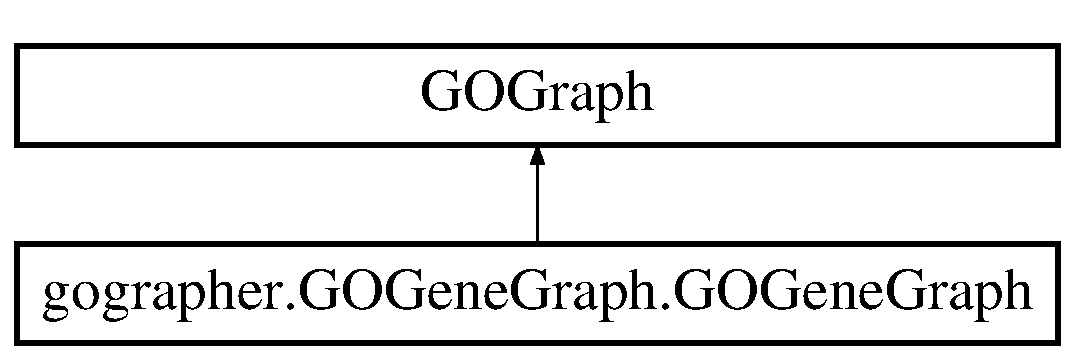
\includegraphics[height=2.000000cm]{classgographer_1_1_g_o_gene_graph_1_1_g_o_gene_graph}
\end{center}
\end{figure}
\subsection*{Public Member Functions}
\begin{DoxyCompactItemize}
\item 
def \hyperlink{classgographer_1_1_g_o_gene_graph_1_1_g_o_gene_graph_a5bda5262ae295bf2f4e299dde69eedb0}{\-\_\-\-\_\-init\-\_\-\-\_\-}
\begin{DoxyCompactList}\small\item\em Create a gene graph from a G\-O\-Graph. \end{DoxyCompactList}\item 
def \hyperlink{classgographer_1_1_g_o_gene_graph_1_1_g_o_gene_graph_ac7a1db7234457886844d399b314bb061}{parse\-Assoc\-File}
\begin{DoxyCompactList}\small\item\em Parses the given association file and adds the gene information to the appropriate nodes. \end{DoxyCompactList}\item 
\hypertarget{classgographer_1_1_g_o_gene_graph_1_1_g_o_gene_graph_a0ce6322f9420cca7b54b6d78a8639454}{def \hyperlink{classgographer_1_1_g_o_gene_graph_1_1_g_o_gene_graph_a0ce6322f9420cca7b54b6d78a8639454}{weight}}\label{classgographer_1_1_g_o_gene_graph_1_1_g_o_gene_graph_a0ce6322f9420cca7b54b6d78a8639454}

\begin{DoxyCompactList}\small\item\em Applies a weight to the graph. \end{DoxyCompactList}\item 
def \hyperlink{classgographer_1_1_g_o_gene_graph_1_1_g_o_gene_graph_aea30558201b976275fa3320e66da9ba3}{to\-G\-O\-Gene\-Pubmed\-Graph}
\begin{DoxyCompactList}\small\item\em Returns a G\-O\-Gene\-Pubmed\-Graph version of itself. \end{DoxyCompactList}\item 
def \hyperlink{classgographer_1_1_g_o_gene_graph_1_1_g_o_gene_graph_a36ebebaac8f9a6fc69dec930bcd57afa}{get\-Genes\-By\-Node}
\begin{DoxyCompactList}\small\item\em Returns the associated genes for a given node. \end{DoxyCompactList}\item 
def \hyperlink{classgographer_1_1_g_o_gene_graph_1_1_g_o_gene_graph_a12623d6d01943b58fd065e622d687f4e}{get\-Propagated\-Genes\-By\-Node}
\begin{DoxyCompactList}\small\item\em Returns the associated propagated genes for a given node. \end{DoxyCompactList}\item 
def \hyperlink{classgographer_1_1_g_o_gene_graph_1_1_g_o_gene_graph_ad5a7be95214be3c6578e295151fe080b}{get\-Nodes\-By\-Gene}
\begin{DoxyCompactList}\small\item\em Returns the associated nodes for a given gene. \end{DoxyCompactList}\item 
\hypertarget{classgographer_1_1_g_o_gene_graph_1_1_g_o_gene_graph_ab0c9a34834a02ea747d4b8826e9ac7fb}{def \hyperlink{classgographer_1_1_g_o_gene_graph_1_1_g_o_gene_graph_ab0c9a34834a02ea747d4b8826e9ac7fb}{propagate\-Genes}}\label{classgographer_1_1_g_o_gene_graph_1_1_g_o_gene_graph_ab0c9a34834a02ea747d4b8826e9ac7fb}

\begin{DoxyCompactList}\small\item\em Propagate the genes associated with each node to its parents. \end{DoxyCompactList}\item 
\hypertarget{classgographer_1_1_g_o_gene_graph_1_1_g_o_gene_graph_a95b66354ebca8636f3837aa8d2e61295}{def {\bfseries remove\-Geneless}}\label{classgographer_1_1_g_o_gene_graph_1_1_g_o_gene_graph_a95b66354ebca8636f3837aa8d2e61295}

\end{DoxyCompactItemize}
\subsection*{Public Attributes}
\begin{DoxyCompactItemize}
\item 
\hypertarget{classgographer_1_1_g_o_gene_graph_1_1_g_o_gene_graph_a1e328c6172de33d810c2878ad17fcb61}{{\bfseries gene\-To\-Node}}\label{classgographer_1_1_g_o_gene_graph_1_1_g_o_gene_graph_a1e328c6172de33d810c2878ad17fcb61}

\item 
\hypertarget{classgographer_1_1_g_o_gene_graph_1_1_g_o_gene_graph_ac7598c02894c42fdf2a80f6ba5d7cfd0}{{\bfseries exclude\-Evidence}}\label{classgographer_1_1_g_o_gene_graph_1_1_g_o_gene_graph_ac7598c02894c42fdf2a80f6ba5d7cfd0}

\end{DoxyCompactItemize}


\subsection{Constructor \& Destructor Documentation}
\hypertarget{classgographer_1_1_g_o_gene_graph_1_1_g_o_gene_graph_a5bda5262ae295bf2f4e299dde69eedb0}{\index{gographer\-::\-G\-O\-Gene\-Graph\-::\-G\-O\-Gene\-Graph@{gographer\-::\-G\-O\-Gene\-Graph\-::\-G\-O\-Gene\-Graph}!\-\_\-\-\_\-init\-\_\-\-\_\-@{\-\_\-\-\_\-init\-\_\-\-\_\-}}
\index{\-\_\-\-\_\-init\-\_\-\-\_\-@{\-\_\-\-\_\-init\-\_\-\-\_\-}!gographer::GOGeneGraph::GOGeneGraph@{gographer\-::\-G\-O\-Gene\-Graph\-::\-G\-O\-Gene\-Graph}}
\subsubsection[{\-\_\-\-\_\-init\-\_\-\-\_\-}]{\setlength{\rightskip}{0pt plus 5cm}def gographer.\-G\-O\-Gene\-Graph.\-G\-O\-Gene\-Graph.\-\_\-\-\_\-init\-\_\-\-\_\- (
\begin{DoxyParamCaption}
\item[{}]{self, }
\item[{}]{gograph, }
\item[{}]{assoc = {\ttfamily None}, }
\item[{}]{exclude\-Evidence = {\ttfamily \mbox{[}\mbox{]}}, }
\item[{}]{types = {\ttfamily \mbox{[}\char`\"{}protein\char`\"{}\mbox{]}}}
\end{DoxyParamCaption}
)}}\label{classgographer_1_1_g_o_gene_graph_1_1_g_o_gene_graph_a5bda5262ae295bf2f4e299dde69eedb0}


Create a gene graph from a G\-O\-Graph. 


\begin{DoxyParams}{Parameters}
{\em gograph} & A G\-O\-Graph to base this graph off of \\
\hline
{\em assoc} & The file containing gene association information \\
\hline
{\em exclude\-Evidence} & A list of the evidence codes that should be ignored \\
\hline
\end{DoxyParams}


\subsection{Member Function Documentation}
\hypertarget{classgographer_1_1_g_o_gene_graph_1_1_g_o_gene_graph_a36ebebaac8f9a6fc69dec930bcd57afa}{\index{gographer\-::\-G\-O\-Gene\-Graph\-::\-G\-O\-Gene\-Graph@{gographer\-::\-G\-O\-Gene\-Graph\-::\-G\-O\-Gene\-Graph}!get\-Genes\-By\-Node@{get\-Genes\-By\-Node}}
\index{get\-Genes\-By\-Node@{get\-Genes\-By\-Node}!gographer::GOGeneGraph::GOGeneGraph@{gographer\-::\-G\-O\-Gene\-Graph\-::\-G\-O\-Gene\-Graph}}
\subsubsection[{get\-Genes\-By\-Node}]{\setlength{\rightskip}{0pt plus 5cm}def gographer.\-G\-O\-Gene\-Graph.\-G\-O\-Gene\-Graph.\-get\-Genes\-By\-Node (
\begin{DoxyParamCaption}
\item[{}]{self, }
\item[{}]{goid}
\end{DoxyParamCaption}
)}}\label{classgographer_1_1_g_o_gene_graph_1_1_g_o_gene_graph_a36ebebaac8f9a6fc69dec930bcd57afa}


Returns the associated genes for a given node. 


\begin{DoxyParams}{Parameters}
{\em goid} & The G\-O\-I\-D of the node to retrieve the associated genes from \\
\hline
\end{DoxyParams}
\hypertarget{classgographer_1_1_g_o_gene_graph_1_1_g_o_gene_graph_ad5a7be95214be3c6578e295151fe080b}{\index{gographer\-::\-G\-O\-Gene\-Graph\-::\-G\-O\-Gene\-Graph@{gographer\-::\-G\-O\-Gene\-Graph\-::\-G\-O\-Gene\-Graph}!get\-Nodes\-By\-Gene@{get\-Nodes\-By\-Gene}}
\index{get\-Nodes\-By\-Gene@{get\-Nodes\-By\-Gene}!gographer::GOGeneGraph::GOGeneGraph@{gographer\-::\-G\-O\-Gene\-Graph\-::\-G\-O\-Gene\-Graph}}
\subsubsection[{get\-Nodes\-By\-Gene}]{\setlength{\rightskip}{0pt plus 5cm}def gographer.\-G\-O\-Gene\-Graph.\-G\-O\-Gene\-Graph.\-get\-Nodes\-By\-Gene (
\begin{DoxyParamCaption}
\item[{}]{self, }
\item[{}]{geneid}
\end{DoxyParamCaption}
)}}\label{classgographer_1_1_g_o_gene_graph_1_1_g_o_gene_graph_ad5a7be95214be3c6578e295151fe080b}


Returns the associated nodes for a given gene. 


\begin{DoxyParams}{Parameters}
{\em geneid} & The I\-D of the gene for which to retrieve the associated nodes \\
\hline
\end{DoxyParams}
\hypertarget{classgographer_1_1_g_o_gene_graph_1_1_g_o_gene_graph_a12623d6d01943b58fd065e622d687f4e}{\index{gographer\-::\-G\-O\-Gene\-Graph\-::\-G\-O\-Gene\-Graph@{gographer\-::\-G\-O\-Gene\-Graph\-::\-G\-O\-Gene\-Graph}!get\-Propagated\-Genes\-By\-Node@{get\-Propagated\-Genes\-By\-Node}}
\index{get\-Propagated\-Genes\-By\-Node@{get\-Propagated\-Genes\-By\-Node}!gographer::GOGeneGraph::GOGeneGraph@{gographer\-::\-G\-O\-Gene\-Graph\-::\-G\-O\-Gene\-Graph}}
\subsubsection[{get\-Propagated\-Genes\-By\-Node}]{\setlength{\rightskip}{0pt plus 5cm}def gographer.\-G\-O\-Gene\-Graph.\-G\-O\-Gene\-Graph.\-get\-Propagated\-Genes\-By\-Node (
\begin{DoxyParamCaption}
\item[{}]{self, }
\item[{}]{goid}
\end{DoxyParamCaption}
)}}\label{classgographer_1_1_g_o_gene_graph_1_1_g_o_gene_graph_a12623d6d01943b58fd065e622d687f4e}


Returns the associated propagated genes for a given node. 


\begin{DoxyParams}{Parameters}
{\em goid} & The G\-O\-I\-D of the node to retrieve the associated propagated genes from \\
\hline
\end{DoxyParams}
\hypertarget{classgographer_1_1_g_o_gene_graph_1_1_g_o_gene_graph_ac7a1db7234457886844d399b314bb061}{\index{gographer\-::\-G\-O\-Gene\-Graph\-::\-G\-O\-Gene\-Graph@{gographer\-::\-G\-O\-Gene\-Graph\-::\-G\-O\-Gene\-Graph}!parse\-Assoc\-File@{parse\-Assoc\-File}}
\index{parse\-Assoc\-File@{parse\-Assoc\-File}!gographer::GOGeneGraph::GOGeneGraph@{gographer\-::\-G\-O\-Gene\-Graph\-::\-G\-O\-Gene\-Graph}}
\subsubsection[{parse\-Assoc\-File}]{\setlength{\rightskip}{0pt plus 5cm}def gographer.\-G\-O\-Gene\-Graph.\-G\-O\-Gene\-Graph.\-parse\-Assoc\-File (
\begin{DoxyParamCaption}
\item[{}]{self, }
\item[{}]{assoc, }
\item[{}]{types = {\ttfamily \mbox{[}\char`\"{}protein\char`\"{}\mbox{]}}}
\end{DoxyParamCaption}
)}}\label{classgographer_1_1_g_o_gene_graph_1_1_g_o_gene_graph_ac7a1db7234457886844d399b314bb061}


Parses the given association file and adds the gene information to the appropriate nodes. 


\begin{DoxyParams}{Parameters}
{\em assoc} & The name of the association file to be parsed \\
\hline
\end{DoxyParams}
\hypertarget{classgographer_1_1_g_o_gene_graph_1_1_g_o_gene_graph_aea30558201b976275fa3320e66da9ba3}{\index{gographer\-::\-G\-O\-Gene\-Graph\-::\-G\-O\-Gene\-Graph@{gographer\-::\-G\-O\-Gene\-Graph\-::\-G\-O\-Gene\-Graph}!to\-G\-O\-Gene\-Pubmed\-Graph@{to\-G\-O\-Gene\-Pubmed\-Graph}}
\index{to\-G\-O\-Gene\-Pubmed\-Graph@{to\-G\-O\-Gene\-Pubmed\-Graph}!gographer::GOGeneGraph::GOGeneGraph@{gographer\-::\-G\-O\-Gene\-Graph\-::\-G\-O\-Gene\-Graph}}
\subsubsection[{to\-G\-O\-Gene\-Pubmed\-Graph}]{\setlength{\rightskip}{0pt plus 5cm}def gographer.\-G\-O\-Gene\-Graph.\-G\-O\-Gene\-Graph.\-to\-G\-O\-Gene\-Pubmed\-Graph (
\begin{DoxyParamCaption}
\item[{}]{self}
\end{DoxyParamCaption}
)}}\label{classgographer_1_1_g_o_gene_graph_1_1_g_o_gene_graph_aea30558201b976275fa3320e66da9ba3}


Returns a G\-O\-Gene\-Pubmed\-Graph version of itself. 


\begin{DoxyParams}{Parameters}
{\em gopubmedgraph} & The G\-O\-Pubmed\-Graph that this graph is to be merged with \\
\hline
\end{DoxyParams}


The documentation for this class was generated from the following file\-:\begin{DoxyCompactItemize}
\item 
/\-Users/\-Zack/\-Desktop/\-Comp\-Sci/cs1680/gographer/G\-O\-Gene\-Graph.\-py\end{DoxyCompactItemize}

\hypertarget{classgographer_1_1_g_o_gene_pubmed_graph_1_1_g_o_gene_pubmed_graph}{\section{gographer.\-G\-O\-Gene\-Pubmed\-Graph.\-G\-O\-Gene\-Pubmed\-Graph Class Reference}
\label{classgographer_1_1_g_o_gene_pubmed_graph_1_1_g_o_gene_pubmed_graph}\index{gographer.\-G\-O\-Gene\-Pubmed\-Graph.\-G\-O\-Gene\-Pubmed\-Graph@{gographer.\-G\-O\-Gene\-Pubmed\-Graph.\-G\-O\-Gene\-Pubmed\-Graph}}
}
Inheritance diagram for gographer.\-G\-O\-Gene\-Pubmed\-Graph.\-G\-O\-Gene\-Pubmed\-Graph\-:\begin{figure}[H]
\begin{center}
\leavevmode
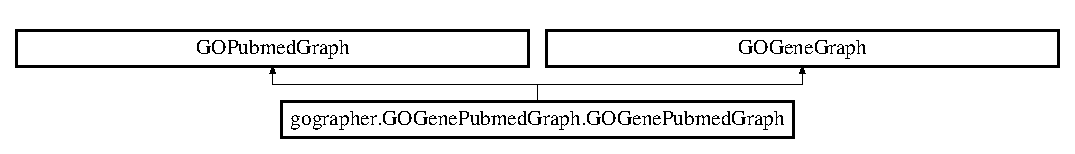
\includegraphics[height=1.623188cm]{classgographer_1_1_g_o_gene_pubmed_graph_1_1_g_o_gene_pubmed_graph}
\end{center}
\end{figure}
\subsection*{Public Member Functions}
\begin{DoxyCompactItemize}
\item 
def \hyperlink{classgographer_1_1_g_o_gene_pubmed_graph_1_1_g_o_gene_pubmed_graph_abfbc7f7350246a08877847e8caaf4a7e}{\-\_\-\-\_\-init\-\_\-\-\_\-}
\begin{DoxyCompactList}\small\item\em Create a gene pubmed graph from a G\-O\-Pubmed\-Graph and G\-O\-Gene\-Graph. \end{DoxyCompactList}\item 
def \hyperlink{classgographer_1_1_g_o_gene_pubmed_graph_1_1_g_o_gene_pubmed_graph_a86edce00d51c5ed23e6f2dbff3edecf6}{parse\-Assoc\-File}
\begin{DoxyCompactList}\small\item\em Parses the given association file and adds the gene and pubmed information to the appropriate nodes. \end{DoxyCompactList}\item 
def \hyperlink{classgographer_1_1_g_o_gene_pubmed_graph_1_1_g_o_gene_pubmed_graph_adb93d9944cbe668abd89f0cbb2eccc8a}{weight\-Nodes}
\begin{DoxyCompactList}\small\item\em Weights the gene pubmed graph based off of the weight factor. \end{DoxyCompactList}\item 
def \hyperlink{classgographer_1_1_g_o_gene_pubmed_graph_1_1_g_o_gene_pubmed_graph_a7b3fe16973f4a2c382098883571c4ec2}{make\-Merged}
\begin{DoxyCompactList}\small\item\em Merges the graph using the selected method. \end{DoxyCompactList}\item 
def \hyperlink{classgographer_1_1_g_o_gene_pubmed_graph_1_1_g_o_gene_pubmed_graph_a0411946b8708273b12b97690c52ce35f}{merge\-Graph\-I\-B}
\begin{DoxyCompactList}\small\item\em Merges the graph, and checks before each merge to ensure the probability of associated information loss is less than the set max probability. \end{DoxyCompactList}\item 
def \hyperlink{classgographer_1_1_g_o_gene_pubmed_graph_1_1_g_o_gene_pubmed_graph_a1c7adf21bb9b5e03699b44da64dd3f75}{merge\-Graph\-Mult}
\begin{DoxyCompactList}\small\item\em Multi-\/\-Graph Merge. \end{DoxyCompactList}\item 
def \hyperlink{classgographer_1_1_g_o_gene_pubmed_graph_1_1_g_o_gene_pubmed_graph_af6522527bb436dfd862d4c60d93c3fa1}{merge\-Augmented}
\begin{DoxyCompactList}\small\item\em Augmented Graph Merge. \end{DoxyCompactList}\item 
def \hyperlink{classgographer_1_1_g_o_gene_pubmed_graph_1_1_g_o_gene_pubmed_graph_a6841cc14cc8e345aec74590fd8302bb9}{get\-Graph\-Info}
\begin{DoxyCompactList}\small\item\em Gets steiner graph and p-\/value. \end{DoxyCompactList}\item 
def \hyperlink{classgographer_1_1_g_o_gene_pubmed_graph_1_1_g_o_gene_pubmed_graph_a421ce63e7d47fd4c4bd1df3e55b8f180}{create\-Di\-Graph\-Copy}
\begin{DoxyCompactList}\small\item\em Creates a Di\-Graph copy of the graph containing only the nodes that annotate, or ancestors of nodes that annotate, the genes of interest. \end{DoxyCompactList}\item 
def \hyperlink{classgographer_1_1_g_o_gene_pubmed_graph_1_1_g_o_gene_pubmed_graph_a3a4964654724f0a716aa5bd98c45c218}{augment\-Graph}
\begin{DoxyCompactList}\small\item\em Adds edges between nodes that share common genes, with the edge weight depending on the number of genes shared. \end{DoxyCompactList}\item 
def \hyperlink{classgographer_1_1_g_o_gene_pubmed_graph_1_1_g_o_gene_pubmed_graph_a8a4f36c28c64041a147f2847e313f94f}{remove\-Empty\-Node}
\begin{DoxyCompactList}\small\item\em Checks and removes the node if it does not contain any directly associated or merged genes, also checks if any newly created leaf nodes are empty and removes them if they are. \end{DoxyCompactList}\item 
\hypertarget{classgographer_1_1_g_o_gene_pubmed_graph_1_1_g_o_gene_pubmed_graph_a4b48cabd6d6d54ac8c6a2471019e8b6c}{def {\bfseries merge\-Graph\-Prob}}\label{classgographer_1_1_g_o_gene_pubmed_graph_1_1_g_o_gene_pubmed_graph_a4b48cabd6d6d54ac8c6a2471019e8b6c}

\end{DoxyCompactItemize}
\subsection*{Public Attributes}
\begin{DoxyCompactItemize}
\item 
\hypertarget{classgographer_1_1_g_o_gene_pubmed_graph_1_1_g_o_gene_pubmed_graph_ab4d15a054d7a19659b8fbff72754ca03}{{\bfseries pubmed\-To\-Node}}\label{classgographer_1_1_g_o_gene_pubmed_graph_1_1_g_o_gene_pubmed_graph_ab4d15a054d7a19659b8fbff72754ca03}

\item 
\hypertarget{classgographer_1_1_g_o_gene_pubmed_graph_1_1_g_o_gene_pubmed_graph_a164b57f5fa534257163cd14092797955}{{\bfseries gene\-To\-Node}}\label{classgographer_1_1_g_o_gene_pubmed_graph_1_1_g_o_gene_pubmed_graph_a164b57f5fa534257163cd14092797955}

\item 
\hypertarget{classgographer_1_1_g_o_gene_pubmed_graph_1_1_g_o_gene_pubmed_graph_ae6f6423d35011c3e564b33a916822809}{{\bfseries exclude\-Evidence}}\label{classgographer_1_1_g_o_gene_pubmed_graph_1_1_g_o_gene_pubmed_graph_ae6f6423d35011c3e564b33a916822809}

\end{DoxyCompactItemize}


\subsection{Constructor \& Destructor Documentation}
\hypertarget{classgographer_1_1_g_o_gene_pubmed_graph_1_1_g_o_gene_pubmed_graph_abfbc7f7350246a08877847e8caaf4a7e}{\index{gographer\-::\-G\-O\-Gene\-Pubmed\-Graph\-::\-G\-O\-Gene\-Pubmed\-Graph@{gographer\-::\-G\-O\-Gene\-Pubmed\-Graph\-::\-G\-O\-Gene\-Pubmed\-Graph}!\-\_\-\-\_\-init\-\_\-\-\_\-@{\-\_\-\-\_\-init\-\_\-\-\_\-}}
\index{\-\_\-\-\_\-init\-\_\-\-\_\-@{\-\_\-\-\_\-init\-\_\-\-\_\-}!gographer::GOGenePubmedGraph::GOGenePubmedGraph@{gographer\-::\-G\-O\-Gene\-Pubmed\-Graph\-::\-G\-O\-Gene\-Pubmed\-Graph}}
\subsubsection[{\-\_\-\-\_\-init\-\_\-\-\_\-}]{\setlength{\rightskip}{0pt plus 5cm}def gographer.\-G\-O\-Gene\-Pubmed\-Graph.\-G\-O\-Gene\-Pubmed\-Graph.\-\_\-\-\_\-init\-\_\-\-\_\- (
\begin{DoxyParamCaption}
\item[{}]{self, }
\item[{}]{gopubmedgraph, }
\item[{}]{gogenegraph}
\end{DoxyParamCaption}
)}}\label{classgographer_1_1_g_o_gene_pubmed_graph_1_1_g_o_gene_pubmed_graph_abfbc7f7350246a08877847e8caaf4a7e}


Create a gene pubmed graph from a G\-O\-Pubmed\-Graph and G\-O\-Gene\-Graph. 


\begin{DoxyParams}{Parameters}
{\em gopubmedgraph} & The G\-O\-Pubmed\-Graph that should be merged to form the gene pubmed graph \\
\hline
{\em gogenegraph} & The G\-O\-Gene\-Graph that should be merged to form the gene pubmed graph \\
\hline
\end{DoxyParams}


\subsection{Member Function Documentation}
\hypertarget{classgographer_1_1_g_o_gene_pubmed_graph_1_1_g_o_gene_pubmed_graph_a3a4964654724f0a716aa5bd98c45c218}{\index{gographer\-::\-G\-O\-Gene\-Pubmed\-Graph\-::\-G\-O\-Gene\-Pubmed\-Graph@{gographer\-::\-G\-O\-Gene\-Pubmed\-Graph\-::\-G\-O\-Gene\-Pubmed\-Graph}!augment\-Graph@{augment\-Graph}}
\index{augment\-Graph@{augment\-Graph}!gographer::GOGenePubmedGraph::GOGenePubmedGraph@{gographer\-::\-G\-O\-Gene\-Pubmed\-Graph\-::\-G\-O\-Gene\-Pubmed\-Graph}}
\subsubsection[{augment\-Graph}]{\setlength{\rightskip}{0pt plus 5cm}def gographer.\-G\-O\-Gene\-Pubmed\-Graph.\-G\-O\-Gene\-Pubmed\-Graph.\-augment\-Graph (
\begin{DoxyParamCaption}
\item[{}]{self, }
\item[{}]{sub\-Graph, }
\item[{}]{term\-List, }
\item[{}]{gene\-Tuples, }
\item[{}]{fifth}
\end{DoxyParamCaption}
)}}\label{classgographer_1_1_g_o_gene_pubmed_graph_1_1_g_o_gene_pubmed_graph_a3a4964654724f0a716aa5bd98c45c218}


Adds edges between nodes that share common genes, with the edge weight depending on the number of genes shared. 


\begin{DoxyParams}{Parameters}
{\em sub\-Graph} & The subgraph of the graph that will be augmented \\
\hline
{\em term\-List} & The list of nodes within the subgraph to check for shared genes \\
\hline
{\em gene\-Tuples} & The genes that re of interest \\
\hline
{\em fifth} & The edge weight that falls within the fifth percentile /return sub\-Graph The augmented subgraph \\
\hline
\end{DoxyParams}
\hypertarget{classgographer_1_1_g_o_gene_pubmed_graph_1_1_g_o_gene_pubmed_graph_a421ce63e7d47fd4c4bd1df3e55b8f180}{\index{gographer\-::\-G\-O\-Gene\-Pubmed\-Graph\-::\-G\-O\-Gene\-Pubmed\-Graph@{gographer\-::\-G\-O\-Gene\-Pubmed\-Graph\-::\-G\-O\-Gene\-Pubmed\-Graph}!create\-Di\-Graph\-Copy@{create\-Di\-Graph\-Copy}}
\index{create\-Di\-Graph\-Copy@{create\-Di\-Graph\-Copy}!gographer::GOGenePubmedGraph::GOGenePubmedGraph@{gographer\-::\-G\-O\-Gene\-Pubmed\-Graph\-::\-G\-O\-Gene\-Pubmed\-Graph}}
\subsubsection[{create\-Di\-Graph\-Copy}]{\setlength{\rightskip}{0pt plus 5cm}def gographer.\-G\-O\-Gene\-Pubmed\-Graph.\-G\-O\-Gene\-Pubmed\-Graph.\-create\-Di\-Graph\-Copy (
\begin{DoxyParamCaption}
\item[{}]{self, }
\item[{}]{gene\-Tuples}
\end{DoxyParamCaption}
)}}\label{classgographer_1_1_g_o_gene_pubmed_graph_1_1_g_o_gene_pubmed_graph_a421ce63e7d47fd4c4bd1df3e55b8f180}


Creates a Di\-Graph copy of the graph containing only the nodes that annotate, or ancestors of nodes that annotate, the genes of interest. 


\begin{DoxyParams}{Parameters}
{\em gene\-Tuples} & The list of genes of interest /return copy\-Graph The created Di\-Graph copy \\
\hline
\end{DoxyParams}
\hypertarget{classgographer_1_1_g_o_gene_pubmed_graph_1_1_g_o_gene_pubmed_graph_a6841cc14cc8e345aec74590fd8302bb9}{\index{gographer\-::\-G\-O\-Gene\-Pubmed\-Graph\-::\-G\-O\-Gene\-Pubmed\-Graph@{gographer\-::\-G\-O\-Gene\-Pubmed\-Graph\-::\-G\-O\-Gene\-Pubmed\-Graph}!get\-Graph\-Info@{get\-Graph\-Info}}
\index{get\-Graph\-Info@{get\-Graph\-Info}!gographer::GOGenePubmedGraph::GOGenePubmedGraph@{gographer\-::\-G\-O\-Gene\-Pubmed\-Graph\-::\-G\-O\-Gene\-Pubmed\-Graph}}
\subsubsection[{get\-Graph\-Info}]{\setlength{\rightskip}{0pt plus 5cm}def gographer.\-G\-O\-Gene\-Pubmed\-Graph.\-G\-O\-Gene\-Pubmed\-Graph.\-get\-Graph\-Info (
\begin{DoxyParamCaption}
\item[{}]{self, }
\item[{}]{model, }
\item[{}]{gene\-List}
\end{DoxyParamCaption}
)}}\label{classgographer_1_1_g_o_gene_pubmed_graph_1_1_g_o_gene_pubmed_graph_a6841cc14cc8e345aec74590fd8302bb9}


Gets steiner graph and p-\/value. 


\begin{DoxyParams}{Parameters}
{\em model} & p-\/value calculation model \\
\hline
{\em gene\-List} & List of input genes \\
\hline
\end{DoxyParams}
\hypertarget{classgographer_1_1_g_o_gene_pubmed_graph_1_1_g_o_gene_pubmed_graph_a7b3fe16973f4a2c382098883571c4ec2}{\index{gographer\-::\-G\-O\-Gene\-Pubmed\-Graph\-::\-G\-O\-Gene\-Pubmed\-Graph@{gographer\-::\-G\-O\-Gene\-Pubmed\-Graph\-::\-G\-O\-Gene\-Pubmed\-Graph}!make\-Merged@{make\-Merged}}
\index{make\-Merged@{make\-Merged}!gographer::GOGenePubmedGraph::GOGenePubmedGraph@{gographer\-::\-G\-O\-Gene\-Pubmed\-Graph\-::\-G\-O\-Gene\-Pubmed\-Graph}}
\subsubsection[{make\-Merged}]{\setlength{\rightskip}{0pt plus 5cm}def gographer.\-G\-O\-Gene\-Pubmed\-Graph.\-G\-O\-Gene\-Pubmed\-Graph.\-make\-Merged (
\begin{DoxyParamCaption}
\item[{}]{self, }
\item[{}]{genes, }
\item[{}]{model, }
\item[{}]{mode = {\ttfamily 'IB'}, }
\item[{}]{max\-Prob = {\ttfamily 0.05}, }
\item[{}]{max\-Merged\-Gene\-Count = {\ttfamily 200}, }
\item[{}]{min\-Gene\-Auto\-Merge = {\ttfamily 5}}
\end{DoxyParamCaption}
)}}\label{classgographer_1_1_g_o_gene_pubmed_graph_1_1_g_o_gene_pubmed_graph_a7b3fe16973f4a2c382098883571c4ec2}


Merges the graph using the selected method. 


\begin{DoxyParams}{Parameters}
{\em genes} & List of genes that should be kept in the graph \\
\hline
{\em mode} & Merging method to be used, default is 'I\-B' \\
\hline
{\em model} & Model used for calculating probability \\
\hline
{\em max\-Prob} & The maximum allowed probability for a merging to occur, the default is 0.\-05 \\
\hline
{\em max\-Merged\-Gene\-Count} & The maximum allowed number of merged genes for any given node, merging stops at that node if the max is reached. The default value is 200 \\
\hline
{\em max\-Gene\-Auto\-Merge} & The maximum number of genes associated with a node for it to be automatically merged \\
\hline
\end{DoxyParams}
\hypertarget{classgographer_1_1_g_o_gene_pubmed_graph_1_1_g_o_gene_pubmed_graph_af6522527bb436dfd862d4c60d93c3fa1}{\index{gographer\-::\-G\-O\-Gene\-Pubmed\-Graph\-::\-G\-O\-Gene\-Pubmed\-Graph@{gographer\-::\-G\-O\-Gene\-Pubmed\-Graph\-::\-G\-O\-Gene\-Pubmed\-Graph}!merge\-Augmented@{merge\-Augmented}}
\index{merge\-Augmented@{merge\-Augmented}!gographer::GOGenePubmedGraph::GOGenePubmedGraph@{gographer\-::\-G\-O\-Gene\-Pubmed\-Graph\-::\-G\-O\-Gene\-Pubmed\-Graph}}
\subsubsection[{merge\-Augmented}]{\setlength{\rightskip}{0pt plus 5cm}def gographer.\-G\-O\-Gene\-Pubmed\-Graph.\-G\-O\-Gene\-Pubmed\-Graph.\-merge\-Augmented (
\begin{DoxyParamCaption}
\item[{}]{self, }
\item[{}]{model, }
\item[{}]{max\-Prob = {\ttfamily 0.05}, }
\item[{}]{max\-Merged\-Gene\-Count = {\ttfamily 200}, }
\item[{}]{min\-Gene\-Auto\-Merge = {\ttfamily 5}, }
\item[{}]{min\-Level = {\ttfamily 0}}
\end{DoxyParamCaption}
)}}\label{classgographer_1_1_g_o_gene_pubmed_graph_1_1_g_o_gene_pubmed_graph_af6522527bb436dfd862d4c60d93c3fa1}


Augmented Graph Merge. 


\begin{DoxyParams}{Parameters}
{\em model} & \\
\hline
{\em max\-Prob} & Always set to 0.\-05 \\
\hline
{\em max\-Merged\-Gene\-Count} & Always set to 200 \\
\hline
{\em min\-Gene\-Auto\-Merge} & Always set to 5 \\
\hline
{\em min\-Level} & Always set to 0 \\
\hline
\end{DoxyParams}
\hypertarget{classgographer_1_1_g_o_gene_pubmed_graph_1_1_g_o_gene_pubmed_graph_a0411946b8708273b12b97690c52ce35f}{\index{gographer\-::\-G\-O\-Gene\-Pubmed\-Graph\-::\-G\-O\-Gene\-Pubmed\-Graph@{gographer\-::\-G\-O\-Gene\-Pubmed\-Graph\-::\-G\-O\-Gene\-Pubmed\-Graph}!merge\-Graph\-I\-B@{merge\-Graph\-I\-B}}
\index{merge\-Graph\-I\-B@{merge\-Graph\-I\-B}!gographer::GOGenePubmedGraph::GOGenePubmedGraph@{gographer\-::\-G\-O\-Gene\-Pubmed\-Graph\-::\-G\-O\-Gene\-Pubmed\-Graph}}
\subsubsection[{merge\-Graph\-I\-B}]{\setlength{\rightskip}{0pt plus 5cm}def gographer.\-G\-O\-Gene\-Pubmed\-Graph.\-G\-O\-Gene\-Pubmed\-Graph.\-merge\-Graph\-I\-B (
\begin{DoxyParamCaption}
\item[{}]{self, }
\item[{}]{model, }
\item[{}]{max\-Prob = {\ttfamily 0.05}, }
\item[{}]{max\-Merged\-Gene\-Count = {\ttfamily 200}, }
\item[{}]{min\-Gene\-Auto\-Merge = {\ttfamily 5}}
\end{DoxyParamCaption}
)}}\label{classgographer_1_1_g_o_gene_pubmed_graph_1_1_g_o_gene_pubmed_graph_a0411946b8708273b12b97690c52ce35f}


Merges the graph, and checks before each merge to ensure the probability of associated information loss is less than the set max probability. 


\begin{DoxyParams}{Parameters}
{\em graph} & A weighted \hyperlink{classgographer_1_1_g_o_gene_pubmed_graph_1_1_g_o_gene_pubmed_graph}{G\-O\-Gene\-Pubmed\-Graph} that will be merged \\
\hline
{\em model} & The model from which to calculate the probability \\
\hline
{\em max\-Prob} & The max allowed probaiblity for a merging to occur, the default value is 0.\-05 \\
\hline
{\em max\-Merged\-Gene\-Count} & The max allowed number of merged genes for any given node, merging stops at that node if the max is reached. The default value is 200 \\
\hline
\end{DoxyParams}
\hypertarget{classgographer_1_1_g_o_gene_pubmed_graph_1_1_g_o_gene_pubmed_graph_a1c7adf21bb9b5e03699b44da64dd3f75}{\index{gographer\-::\-G\-O\-Gene\-Pubmed\-Graph\-::\-G\-O\-Gene\-Pubmed\-Graph@{gographer\-::\-G\-O\-Gene\-Pubmed\-Graph\-::\-G\-O\-Gene\-Pubmed\-Graph}!merge\-Graph\-Mult@{merge\-Graph\-Mult}}
\index{merge\-Graph\-Mult@{merge\-Graph\-Mult}!gographer::GOGenePubmedGraph::GOGenePubmedGraph@{gographer\-::\-G\-O\-Gene\-Pubmed\-Graph\-::\-G\-O\-Gene\-Pubmed\-Graph}}
\subsubsection[{merge\-Graph\-Mult}]{\setlength{\rightskip}{0pt plus 5cm}def gographer.\-G\-O\-Gene\-Pubmed\-Graph.\-G\-O\-Gene\-Pubmed\-Graph.\-merge\-Graph\-Mult (
\begin{DoxyParamCaption}
\item[{}]{self, }
\item[{}]{model, }
\item[{}]{max\-Prob = {\ttfamily 0.05}, }
\item[{}]{max\-Merged\-Gene\-Count = {\ttfamily 200}, }
\item[{}]{min\-Gene\-Auto\-Merge = {\ttfamily 5}}
\end{DoxyParamCaption}
)}}\label{classgographer_1_1_g_o_gene_pubmed_graph_1_1_g_o_gene_pubmed_graph_a1c7adf21bb9b5e03699b44da64dd3f75}


Multi-\/\-Graph Merge. 


\begin{DoxyParams}{Parameters}
{\em model} & \\
\hline
{\em max\-Prob} & Always set to 0.\-05 \\
\hline
{\em max\-Merged\-Gene\-Count} & Always set to 200 \\
\hline
{\em min\-Gene\-Auto\-Merge} & Always set to 5 \\
\hline
\end{DoxyParams}
\hypertarget{classgographer_1_1_g_o_gene_pubmed_graph_1_1_g_o_gene_pubmed_graph_a86edce00d51c5ed23e6f2dbff3edecf6}{\index{gographer\-::\-G\-O\-Gene\-Pubmed\-Graph\-::\-G\-O\-Gene\-Pubmed\-Graph@{gographer\-::\-G\-O\-Gene\-Pubmed\-Graph\-::\-G\-O\-Gene\-Pubmed\-Graph}!parse\-Assoc\-File@{parse\-Assoc\-File}}
\index{parse\-Assoc\-File@{parse\-Assoc\-File}!gographer::GOGenePubmedGraph::GOGenePubmedGraph@{gographer\-::\-G\-O\-Gene\-Pubmed\-Graph\-::\-G\-O\-Gene\-Pubmed\-Graph}}
\subsubsection[{parse\-Assoc\-File}]{\setlength{\rightskip}{0pt plus 5cm}def gographer.\-G\-O\-Gene\-Pubmed\-Graph.\-G\-O\-Gene\-Pubmed\-Graph.\-parse\-Assoc\-File (
\begin{DoxyParamCaption}
\item[{}]{self, }
\item[{}]{assoc, }
\item[{}]{types = {\ttfamily \mbox{[}\char`\"{}protein\char`\"{}\mbox{]}}}
\end{DoxyParamCaption}
)}}\label{classgographer_1_1_g_o_gene_pubmed_graph_1_1_g_o_gene_pubmed_graph_a86edce00d51c5ed23e6f2dbff3edecf6}


Parses the given association file and adds the gene and pubmed information to the appropriate nodes. 


\begin{DoxyParams}{Parameters}
{\em assoc} & The name of the association file to be parsed \\
\hline
\end{DoxyParams}
\hypertarget{classgographer_1_1_g_o_gene_pubmed_graph_1_1_g_o_gene_pubmed_graph_a8a4f36c28c64041a147f2847e313f94f}{\index{gographer\-::\-G\-O\-Gene\-Pubmed\-Graph\-::\-G\-O\-Gene\-Pubmed\-Graph@{gographer\-::\-G\-O\-Gene\-Pubmed\-Graph\-::\-G\-O\-Gene\-Pubmed\-Graph}!remove\-Empty\-Node@{remove\-Empty\-Node}}
\index{remove\-Empty\-Node@{remove\-Empty\-Node}!gographer::GOGenePubmedGraph::GOGenePubmedGraph@{gographer\-::\-G\-O\-Gene\-Pubmed\-Graph\-::\-G\-O\-Gene\-Pubmed\-Graph}}
\subsubsection[{remove\-Empty\-Node}]{\setlength{\rightskip}{0pt plus 5cm}def gographer.\-G\-O\-Gene\-Pubmed\-Graph.\-G\-O\-Gene\-Pubmed\-Graph.\-remove\-Empty\-Node (
\begin{DoxyParamCaption}
\item[{}]{self, }
\item[{}]{node}
\end{DoxyParamCaption}
)}}\label{classgographer_1_1_g_o_gene_pubmed_graph_1_1_g_o_gene_pubmed_graph_a8a4f36c28c64041a147f2847e313f94f}


Checks and removes the node if it does not contain any directly associated or merged genes, also checks if any newly created leaf nodes are empty and removes them if they are. 


\begin{DoxyParams}{Parameters}
{\em node} & The node that will be checked /return graph The updated version of the inputted graph \\
\hline
\end{DoxyParams}
\hypertarget{classgographer_1_1_g_o_gene_pubmed_graph_1_1_g_o_gene_pubmed_graph_adb93d9944cbe668abd89f0cbb2eccc8a}{\index{gographer\-::\-G\-O\-Gene\-Pubmed\-Graph\-::\-G\-O\-Gene\-Pubmed\-Graph@{gographer\-::\-G\-O\-Gene\-Pubmed\-Graph\-::\-G\-O\-Gene\-Pubmed\-Graph}!weight\-Nodes@{weight\-Nodes}}
\index{weight\-Nodes@{weight\-Nodes}!gographer::GOGenePubmedGraph::GOGenePubmedGraph@{gographer\-::\-G\-O\-Gene\-Pubmed\-Graph\-::\-G\-O\-Gene\-Pubmed\-Graph}}
\subsubsection[{weight\-Nodes}]{\setlength{\rightskip}{0pt plus 5cm}def gographer.\-G\-O\-Gene\-Pubmed\-Graph.\-G\-O\-Gene\-Pubmed\-Graph.\-weight\-Nodes (
\begin{DoxyParamCaption}
\item[{}]{self, }
\item[{}]{weighter}
\end{DoxyParamCaption}
)}}\label{classgographer_1_1_g_o_gene_pubmed_graph_1_1_g_o_gene_pubmed_graph_adb93d9944cbe668abd89f0cbb2eccc8a}


Weights the gene pubmed graph based off of the weight factor. 


\begin{DoxyParams}{Parameters}
{\em weighter} & The weighing method by which the proteins and semantic distances should be weighted \\
\hline
\end{DoxyParams}


The documentation for this class was generated from the following file\-:\begin{DoxyCompactItemize}
\item 
/\-Users/\-Zack/\-Desktop/\-Comp\-Sci/cs1680/gographer/G\-O\-Gene\-Pubmed\-Graph.\-py\end{DoxyCompactItemize}

\hypertarget{classgographer_1_1_g_o_graph_1_1_g_o_graph}{\section{gographer.\-G\-O\-Graph.\-G\-O\-Graph Class Reference}
\label{classgographer_1_1_g_o_graph_1_1_g_o_graph}\index{gographer.\-G\-O\-Graph.\-G\-O\-Graph@{gographer.\-G\-O\-Graph.\-G\-O\-Graph}}
}
Inheritance diagram for gographer.\-G\-O\-Graph.\-G\-O\-Graph\-:\begin{figure}[H]
\begin{center}
\leavevmode
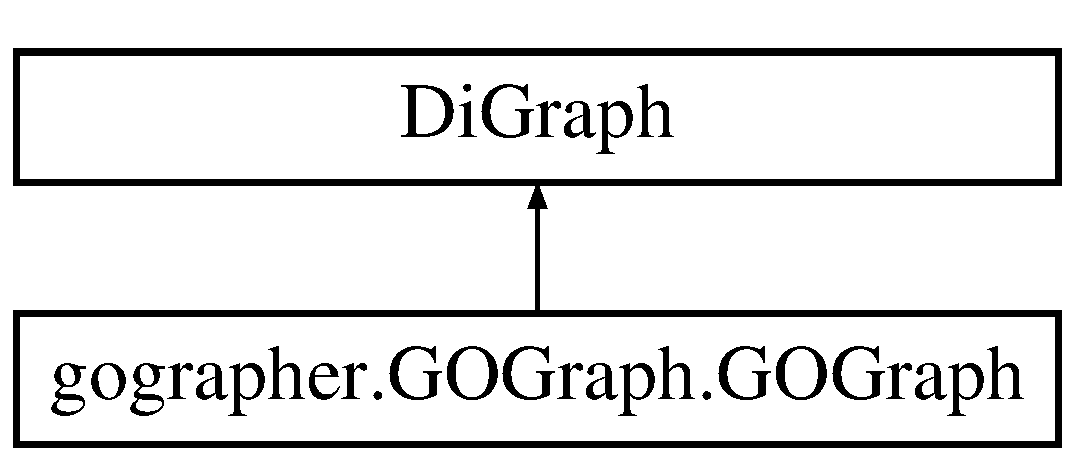
\includegraphics[height=2.000000cm]{classgographer_1_1_g_o_graph_1_1_g_o_graph}
\end{center}
\end{figure}
\subsection*{Public Member Functions}
\begin{DoxyCompactItemize}
\item 
def \hyperlink{classgographer_1_1_g_o_graph_1_1_g_o_graph_a24d8db0ef400bef39324bc804fa34eb4}{\-\_\-\-\_\-init\-\_\-\-\_\-}
\begin{DoxyCompactList}\small\item\em Constructor. \end{DoxyCompactList}\item 
def \hyperlink{classgographer_1_1_g_o_graph_1_1_g_o_graph_acb1ecdd7498c7fcfbfe916fcf73e675a}{parse\-Obo\-Xml}
\begin{DoxyCompactList}\small\item\em Parses the given O\-B\-O X\-M\-L file and creates a \hyperlink{classgographer_1_1_g_o_graph_1_1_g_o_graph}{G\-O\-Graph}. \end{DoxyCompactList}\item 
def \hyperlink{classgographer_1_1_g_o_graph_1_1_g_o_graph_af470097f7034f398a1d77576f1900358}{get\-Level}
\begin{DoxyCompactList}\small\item\em Returns the minimum depth of the node. \end{DoxyCompactList}\item 
\hypertarget{classgographer_1_1_g_o_graph_1_1_g_o_graph_a28ed46813dc6e35385084853cd48ce13}{def \hyperlink{classgographer_1_1_g_o_graph_1_1_g_o_graph_a28ed46813dc6e35385084853cd48ce13}{get\-Name\-Space}}\label{classgographer_1_1_g_o_graph_1_1_g_o_graph_a28ed46813dc6e35385084853cd48ce13}

\begin{DoxyCompactList}\small\item\em Returns the namespace of the graph. \end{DoxyCompactList}\item 
def \hyperlink{classgographer_1_1_g_o_graph_1_1_g_o_graph_a1f0fa0879611bf23be5977bdff1e29d7}{save\-Pickle}
\begin{DoxyCompactList}\small\item\em Save self using pickle protocol. \end{DoxyCompactList}\item 
def \hyperlink{classgographer_1_1_g_o_graph_1_1_g_o_graph_accda51360f6e55aeb466ab84c11877fc}{load\-Pickle}
\begin{DoxyCompactList}\small\item\em Load a pickle from the filesystem. \end{DoxyCompactList}\item 
def \hyperlink{classgographer_1_1_g_o_graph_1_1_g_o_graph_a3770da07e30351e6cee836badfd81a6d}{get\-Node\-Description}
\begin{DoxyCompactList}\small\item\em Get the description of a node. \end{DoxyCompactList}\item 
def \hyperlink{classgographer_1_1_g_o_graph_1_1_g_o_graph_adcde4047692fb0006926fd45692404ba}{get\-Node\-Namespace}
\begin{DoxyCompactList}\small\item\em Get the description of a node. \end{DoxyCompactList}\item 
\hypertarget{classgographer_1_1_g_o_graph_1_1_g_o_graph_a7c7b036c555bf226c7d0877cd15e2dee}{def \hyperlink{classgographer_1_1_g_o_graph_1_1_g_o_graph_a7c7b036c555bf226c7d0877cd15e2dee}{calc\-Descendant\-Count}}\label{classgographer_1_1_g_o_graph_1_1_g_o_graph_a7c7b036c555bf226c7d0877cd15e2dee}

\begin{DoxyCompactList}\small\item\em Calculates and stores the number of descendants each node in the graph has. \end{DoxyCompactList}\item 
def \hyperlink{classgographer_1_1_g_o_graph_1_1_g_o_graph_a12134f0c734684a4947b833e933c927e}{get\-Descendant\-Count}
\begin{DoxyCompactList}\small\item\em Return the number of descendants of the given node. \end{DoxyCompactList}\end{DoxyCompactItemize}
\subsection*{Public Attributes}
\begin{DoxyCompactItemize}
\item 
\hypertarget{classgographer_1_1_g_o_graph_1_1_g_o_graph_a296e0699b66961479b4d715ffccdc1c0}{{\bfseries namespace}}\label{classgographer_1_1_g_o_graph_1_1_g_o_graph_a296e0699b66961479b4d715ffccdc1c0}

\end{DoxyCompactItemize}


\subsection{Constructor \& Destructor Documentation}
\hypertarget{classgographer_1_1_g_o_graph_1_1_g_o_graph_a24d8db0ef400bef39324bc804fa34eb4}{\index{gographer\-::\-G\-O\-Graph\-::\-G\-O\-Graph@{gographer\-::\-G\-O\-Graph\-::\-G\-O\-Graph}!\-\_\-\-\_\-init\-\_\-\-\_\-@{\-\_\-\-\_\-init\-\_\-\-\_\-}}
\index{\-\_\-\-\_\-init\-\_\-\-\_\-@{\-\_\-\-\_\-init\-\_\-\-\_\-}!gographer::GOGraph::GOGraph@{gographer\-::\-G\-O\-Graph\-::\-G\-O\-Graph}}
\subsubsection[{\-\_\-\-\_\-init\-\_\-\-\_\-}]{\setlength{\rightskip}{0pt plus 5cm}def gographer.\-G\-O\-Graph.\-G\-O\-Graph.\-\_\-\-\_\-init\-\_\-\-\_\- (
\begin{DoxyParamCaption}
\item[{}]{self, }
\item[{}]{namespace = {\ttfamily None}, }
\item[{}]{G\-O\-Obo\-Xml\-File\-Name = {\ttfamily None}}
\end{DoxyParamCaption}
)}}\label{classgographer_1_1_g_o_graph_1_1_g_o_graph_a24d8db0ef400bef39324bc804fa34eb4}


Constructor. 


\begin{DoxyParams}{Parameters}
{\em namespace} & The branch of the G\-O ontology stored by this graph \\
\hline
{\em X\-M\-L\-File\-Name} & The file contains the G\-O definition in the format of the O\-B\-O in X\-M\-L \\
\hline
\end{DoxyParams}


\subsection{Member Function Documentation}
\hypertarget{classgographer_1_1_g_o_graph_1_1_g_o_graph_a12134f0c734684a4947b833e933c927e}{\index{gographer\-::\-G\-O\-Graph\-::\-G\-O\-Graph@{gographer\-::\-G\-O\-Graph\-::\-G\-O\-Graph}!get\-Descendant\-Count@{get\-Descendant\-Count}}
\index{get\-Descendant\-Count@{get\-Descendant\-Count}!gographer::GOGraph::GOGraph@{gographer\-::\-G\-O\-Graph\-::\-G\-O\-Graph}}
\subsubsection[{get\-Descendant\-Count}]{\setlength{\rightskip}{0pt plus 5cm}def gographer.\-G\-O\-Graph.\-G\-O\-Graph.\-get\-Descendant\-Count (
\begin{DoxyParamCaption}
\item[{}]{self, }
\item[{}]{goid}
\end{DoxyParamCaption}
)}}\label{classgographer_1_1_g_o_graph_1_1_g_o_graph_a12134f0c734684a4947b833e933c927e}


Return the number of descendants of the given node. 

Calculates the count if it had not already been done so 
\begin{DoxyParams}{Parameters}
{\em goid} & The G\-O I\-D of the node to return the descendant count of \\
\hline
\end{DoxyParams}
\hypertarget{classgographer_1_1_g_o_graph_1_1_g_o_graph_af470097f7034f398a1d77576f1900358}{\index{gographer\-::\-G\-O\-Graph\-::\-G\-O\-Graph@{gographer\-::\-G\-O\-Graph\-::\-G\-O\-Graph}!get\-Level@{get\-Level}}
\index{get\-Level@{get\-Level}!gographer::GOGraph::GOGraph@{gographer\-::\-G\-O\-Graph\-::\-G\-O\-Graph}}
\subsubsection[{get\-Level}]{\setlength{\rightskip}{0pt plus 5cm}def gographer.\-G\-O\-Graph.\-G\-O\-Graph.\-get\-Level (
\begin{DoxyParamCaption}
\item[{}]{self, }
\item[{}]{goid}
\end{DoxyParamCaption}
)}}\label{classgographer_1_1_g_o_graph_1_1_g_o_graph_af470097f7034f398a1d77576f1900358}


Returns the minimum depth of the node. 


\begin{DoxyParams}{Parameters}
{\em goid} & The G\-O I\-D of the node whose depth will be found and returned \\
\hline
\end{DoxyParams}
\hypertarget{classgographer_1_1_g_o_graph_1_1_g_o_graph_a3770da07e30351e6cee836badfd81a6d}{\index{gographer\-::\-G\-O\-Graph\-::\-G\-O\-Graph@{gographer\-::\-G\-O\-Graph\-::\-G\-O\-Graph}!get\-Node\-Description@{get\-Node\-Description}}
\index{get\-Node\-Description@{get\-Node\-Description}!gographer::GOGraph::GOGraph@{gographer\-::\-G\-O\-Graph\-::\-G\-O\-Graph}}
\subsubsection[{get\-Node\-Description}]{\setlength{\rightskip}{0pt plus 5cm}def gographer.\-G\-O\-Graph.\-G\-O\-Graph.\-get\-Node\-Description (
\begin{DoxyParamCaption}
\item[{}]{self, }
\item[{}]{goid}
\end{DoxyParamCaption}
)}}\label{classgographer_1_1_g_o_graph_1_1_g_o_graph_a3770da07e30351e6cee836badfd81a6d}


Get the description of a node. 


\begin{DoxyParams}{Parameters}
{\em goid} & The G\-O I\-D of the node to get the description of \\
\hline
\end{DoxyParams}
\hypertarget{classgographer_1_1_g_o_graph_1_1_g_o_graph_adcde4047692fb0006926fd45692404ba}{\index{gographer\-::\-G\-O\-Graph\-::\-G\-O\-Graph@{gographer\-::\-G\-O\-Graph\-::\-G\-O\-Graph}!get\-Node\-Namespace@{get\-Node\-Namespace}}
\index{get\-Node\-Namespace@{get\-Node\-Namespace}!gographer::GOGraph::GOGraph@{gographer\-::\-G\-O\-Graph\-::\-G\-O\-Graph}}
\subsubsection[{get\-Node\-Namespace}]{\setlength{\rightskip}{0pt plus 5cm}def gographer.\-G\-O\-Graph.\-G\-O\-Graph.\-get\-Node\-Namespace (
\begin{DoxyParamCaption}
\item[{}]{self, }
\item[{}]{goid}
\end{DoxyParamCaption}
)}}\label{classgographer_1_1_g_o_graph_1_1_g_o_graph_adcde4047692fb0006926fd45692404ba}


Get the description of a node. 


\begin{DoxyParams}{Parameters}
{\em goid} & The G\-O I\-D of the node to get the description of \\
\hline
\end{DoxyParams}
\hypertarget{classgographer_1_1_g_o_graph_1_1_g_o_graph_accda51360f6e55aeb466ab84c11877fc}{\index{gographer\-::\-G\-O\-Graph\-::\-G\-O\-Graph@{gographer\-::\-G\-O\-Graph\-::\-G\-O\-Graph}!load\-Pickle@{load\-Pickle}}
\index{load\-Pickle@{load\-Pickle}!gographer::GOGraph::GOGraph@{gographer\-::\-G\-O\-Graph\-::\-G\-O\-Graph}}
\subsubsection[{load\-Pickle}]{\setlength{\rightskip}{0pt plus 5cm}def gographer.\-G\-O\-Graph.\-G\-O\-Graph.\-load\-Pickle (
\begin{DoxyParamCaption}
\item[{}]{klass, }
\item[{}]{filename = {\ttfamily \char`\"{}gograph.pickle\char`\"{}}}
\end{DoxyParamCaption}
)}}\label{classgographer_1_1_g_o_graph_1_1_g_o_graph_accda51360f6e55aeb466ab84c11877fc}


Load a pickle from the filesystem. 


\begin{DoxyParams}{Parameters}
{\em filename} & The location of the pickle file to load \\
\hline
\end{DoxyParams}
\hypertarget{classgographer_1_1_g_o_graph_1_1_g_o_graph_acb1ecdd7498c7fcfbfe916fcf73e675a}{\index{gographer\-::\-G\-O\-Graph\-::\-G\-O\-Graph@{gographer\-::\-G\-O\-Graph\-::\-G\-O\-Graph}!parse\-Obo\-Xml@{parse\-Obo\-Xml}}
\index{parse\-Obo\-Xml@{parse\-Obo\-Xml}!gographer::GOGraph::GOGraph@{gographer\-::\-G\-O\-Graph\-::\-G\-O\-Graph}}
\subsubsection[{parse\-Obo\-Xml}]{\setlength{\rightskip}{0pt plus 5cm}def gographer.\-G\-O\-Graph.\-G\-O\-Graph.\-parse\-Obo\-Xml (
\begin{DoxyParamCaption}
\item[{}]{self, }
\item[{}]{G\-O\-Obo\-Xml\-File\-Name}
\end{DoxyParamCaption}
)}}\label{classgographer_1_1_g_o_graph_1_1_g_o_graph_acb1ecdd7498c7fcfbfe916fcf73e675a}


Parses the given O\-B\-O X\-M\-L file and creates a \hyperlink{classgographer_1_1_g_o_graph_1_1_g_o_graph}{G\-O\-Graph}. 


\begin{DoxyParams}{Parameters}
{\em G\-O\-Obo\-X\-M\-L\-File\-Name} & The name of the O\-B\-O X\-M\-L file to be parsed \\
\hline
\end{DoxyParams}
\hypertarget{classgographer_1_1_g_o_graph_1_1_g_o_graph_a1f0fa0879611bf23be5977bdff1e29d7}{\index{gographer\-::\-G\-O\-Graph\-::\-G\-O\-Graph@{gographer\-::\-G\-O\-Graph\-::\-G\-O\-Graph}!save\-Pickle@{save\-Pickle}}
\index{save\-Pickle@{save\-Pickle}!gographer::GOGraph::GOGraph@{gographer\-::\-G\-O\-Graph\-::\-G\-O\-Graph}}
\subsubsection[{save\-Pickle}]{\setlength{\rightskip}{0pt plus 5cm}def gographer.\-G\-O\-Graph.\-G\-O\-Graph.\-save\-Pickle (
\begin{DoxyParamCaption}
\item[{}]{self, }
\item[{}]{filename = {\ttfamily \char`\"{}gograph.pickle\char`\"{}}}
\end{DoxyParamCaption}
)}}\label{classgographer_1_1_g_o_graph_1_1_g_o_graph_a1f0fa0879611bf23be5977bdff1e29d7}


Save self using pickle protocol. 


\begin{DoxyParams}{Parameters}
{\em filename} & The filename of the pickle to use \\
\hline
\end{DoxyParams}


The documentation for this class was generated from the following file\-:\begin{DoxyCompactItemize}
\item 
/\-Users/\-Zack/\-Desktop/\-Comp\-Sci/cs1680/gographer/G\-O\-Graph.\-py\end{DoxyCompactItemize}

\hypertarget{classgographer_1_1_g_o_node_1_1_g_o_node}{\section{gographer.\-G\-O\-Node.\-G\-O\-Node Class Reference}
\label{classgographer_1_1_g_o_node_1_1_g_o_node}\index{gographer.\-G\-O\-Node.\-G\-O\-Node@{gographer.\-G\-O\-Node.\-G\-O\-Node}}
}
\subsection*{Public Member Functions}
\begin{DoxyCompactItemize}
\item 
\hypertarget{classgographer_1_1_g_o_node_1_1_g_o_node_ab82e5a00ea9b9a6c42be57512a95d5c1}{def {\bfseries \-\_\-\-\_\-init\-\_\-\-\_\-}}\label{classgographer_1_1_g_o_node_1_1_g_o_node_ab82e5a00ea9b9a6c42be57512a95d5c1}

\item 
def \hyperlink{classgographer_1_1_g_o_node_1_1_g_o_node_aad9563bd645b56b9dd16e425734c41b3}{set\-G\-O\-I\-D}
\begin{DoxyCompactList}\small\item\em Set the G\-O I\-D of the node. \end{DoxyCompactList}\item 
\hypertarget{classgographer_1_1_g_o_node_1_1_g_o_node_a26b818661d7d836fff2e813a846f4f4e}{def \hyperlink{classgographer_1_1_g_o_node_1_1_g_o_node_a26b818661d7d836fff2e813a846f4f4e}{get\-G\-O\-I\-D}}\label{classgographer_1_1_g_o_node_1_1_g_o_node_a26b818661d7d836fff2e813a846f4f4e}

\begin{DoxyCompactList}\small\item\em Returns the G\-O I\-D of the node. \end{DoxyCompactList}\item 
def \hyperlink{classgographer_1_1_g_o_node_1_1_g_o_node_a93c1d2b3080639b2159b81998187b8c3}{set\-Namespace}
\begin{DoxyCompactList}\small\item\em Set the namespace of the node. \end{DoxyCompactList}\item 
\hypertarget{classgographer_1_1_g_o_node_1_1_g_o_node_a8ef6fa408a68319d95fb2488753fd5fc}{def \hyperlink{classgographer_1_1_g_o_node_1_1_g_o_node_a8ef6fa408a68319d95fb2488753fd5fc}{get\-Namespace}}\label{classgographer_1_1_g_o_node_1_1_g_o_node_a8ef6fa408a68319d95fb2488753fd5fc}

\begin{DoxyCompactList}\small\item\em Returns the namespace of the node. \end{DoxyCompactList}\item 
def \hyperlink{classgographer_1_1_g_o_node_1_1_g_o_node_ae99aa1efe2438fc3c971d6f7718943b4}{set\-Parents}
\begin{DoxyCompactList}\small\item\em Set the parents of the node. \end{DoxyCompactList}\item 
\hypertarget{classgographer_1_1_g_o_node_1_1_g_o_node_a3cd34159abd352b56c25dececb1fbe5d}{def \hyperlink{classgographer_1_1_g_o_node_1_1_g_o_node_a3cd34159abd352b56c25dececb1fbe5d}{get\-Parents}}\label{classgographer_1_1_g_o_node_1_1_g_o_node_a3cd34159abd352b56c25dececb1fbe5d}

\begin{DoxyCompactList}\small\item\em Returns the parents of the node. \end{DoxyCompactList}\item 
def \hyperlink{classgographer_1_1_g_o_node_1_1_g_o_node_a82b8251a7dd9698728a4640679242663}{set\-Obsolete}
\begin{DoxyCompactList}\small\item\em Set the obsolete status of the node. \end{DoxyCompactList}\item 
\hypertarget{classgographer_1_1_g_o_node_1_1_g_o_node_aa6a0d9f76513f8dea1d9e3b8a26654e8}{def \hyperlink{classgographer_1_1_g_o_node_1_1_g_o_node_aa6a0d9f76513f8dea1d9e3b8a26654e8}{get\-Obsolete}}\label{classgographer_1_1_g_o_node_1_1_g_o_node_aa6a0d9f76513f8dea1d9e3b8a26654e8}

\begin{DoxyCompactList}\small\item\em Returns the obsolete status of the node (whether or not the term is obsolete) \end{DoxyCompactList}\item 
def \hyperlink{classgographer_1_1_g_o_node_1_1_g_o_node_afb34878daea4862be2712452aa901d65}{set\-Name}
\begin{DoxyCompactList}\small\item\em Set the name of the node. \end{DoxyCompactList}\item 
\hypertarget{classgographer_1_1_g_o_node_1_1_g_o_node_ab2c001a8212e96502b53863d910f2c49}{def \hyperlink{classgographer_1_1_g_o_node_1_1_g_o_node_ab2c001a8212e96502b53863d910f2c49}{get\-Name}}\label{classgographer_1_1_g_o_node_1_1_g_o_node_ab2c001a8212e96502b53863d910f2c49}

\begin{DoxyCompactList}\small\item\em Returns the name of the node. \end{DoxyCompactList}\item 
def \hyperlink{classgographer_1_1_g_o_node_1_1_g_o_node_a7d0ca3ef76b7d2ea93cfaab7dc202e4f}{set\-Description}
\begin{DoxyCompactList}\small\item\em Set the description of the node. \end{DoxyCompactList}\item 
\hypertarget{classgographer_1_1_g_o_node_1_1_g_o_node_a9b05c66b0272bd0453a439fecb435845}{def \hyperlink{classgographer_1_1_g_o_node_1_1_g_o_node_a9b05c66b0272bd0453a439fecb435845}{get\-Description}}\label{classgographer_1_1_g_o_node_1_1_g_o_node_a9b05c66b0272bd0453a439fecb435845}

\begin{DoxyCompactList}\small\item\em Returns the description of the node. \end{DoxyCompactList}\item 
def \hyperlink{classgographer_1_1_g_o_node_1_1_g_o_node_acab0337312c51990cc12d8a5c3a3ef56}{set\-P\-M\-I\-Ds}
\begin{DoxyCompactList}\small\item\em Set the Pub\-Med I\-Ds associated with the node. \end{DoxyCompactList}\item 
\hypertarget{classgographer_1_1_g_o_node_1_1_g_o_node_aa5d4700b9914f7cdb00f2538b83e6b4d}{def \hyperlink{classgographer_1_1_g_o_node_1_1_g_o_node_aa5d4700b9914f7cdb00f2538b83e6b4d}{get\-P\-M\-I\-Ds}}\label{classgographer_1_1_g_o_node_1_1_g_o_node_aa5d4700b9914f7cdb00f2538b83e6b4d}

\begin{DoxyCompactList}\small\item\em Returns the Pub\-Med I\-Ds associated with the node. \end{DoxyCompactList}\item 
def \hyperlink{classgographer_1_1_g_o_node_1_1_g_o_node_a74974a9de346f4fc20c706be06d942ef}{add\-P\-M\-I\-Ds}
\begin{DoxyCompactList}\small\item\em Adds list containing one or more Pub\-Med I\-D tuples to the existing set of Pub\-Med I\-Ds. \end{DoxyCompactList}\item 
def \hyperlink{classgographer_1_1_g_o_node_1_1_g_o_node_a4cb9c3ea2f23af472e15cfc53602cfb8}{set\-Propagated\-P\-M\-I\-Ds}
\begin{DoxyCompactList}\small\item\em Set the propagated Pub\-Med I\-Ds associated with the node or its descendants. \end{DoxyCompactList}\item 
\hypertarget{classgographer_1_1_g_o_node_1_1_g_o_node_ade1c13780ac26daec9341a9db6be26dc}{def \hyperlink{classgographer_1_1_g_o_node_1_1_g_o_node_ade1c13780ac26daec9341a9db6be26dc}{get\-Propagated\-P\-M\-I\-Ds}}\label{classgographer_1_1_g_o_node_1_1_g_o_node_ade1c13780ac26daec9341a9db6be26dc}

\begin{DoxyCompactList}\small\item\em Returns the propagated Pub\-Med I\-Ds associated with the node or its descendants. \end{DoxyCompactList}\item 
def \hyperlink{classgographer_1_1_g_o_node_1_1_g_o_node_ac393afb81160458d096b41f6837e981e}{add\-Propagated\-P\-M\-I\-Ds}
\begin{DoxyCompactList}\small\item\em Adds list containing Pub\-Med I\-D tuples to the existing set of propagated Pub\-Med I\-Ds. \end{DoxyCompactList}\item 
def \hyperlink{classgographer_1_1_g_o_node_1_1_g_o_node_a8085440f2f60e68acc0d436030642671}{set\-Genes}
\begin{DoxyCompactList}\small\item\em Set the genes associated with the node. \end{DoxyCompactList}\item 
\hypertarget{classgographer_1_1_g_o_node_1_1_g_o_node_a1d056c7237ce4d4919d0ad5f5ed4e385}{def \hyperlink{classgographer_1_1_g_o_node_1_1_g_o_node_a1d056c7237ce4d4919d0ad5f5ed4e385}{get\-Genes}}\label{classgographer_1_1_g_o_node_1_1_g_o_node_a1d056c7237ce4d4919d0ad5f5ed4e385}

\begin{DoxyCompactList}\small\item\em Returns the genes associated with the node. \end{DoxyCompactList}\item 
def \hyperlink{classgographer_1_1_g_o_node_1_1_g_o_node_a35be18174f995d9e7db5d23c9cc33189}{add\-Genes}
\begin{DoxyCompactList}\small\item\em Adds list containing one or more gene tuples to the existing set of genes. \end{DoxyCompactList}\item 
def \hyperlink{classgographer_1_1_g_o_node_1_1_g_o_node_aca565668e8254fcf8f360c2600d0f46a}{set\-Propagated\-Genes}
\begin{DoxyCompactList}\small\item\em Set the propagated genes associated with the node or its descendants. \end{DoxyCompactList}\item 
\hypertarget{classgographer_1_1_g_o_node_1_1_g_o_node_a6cf34da2a1bc2b352bc9afa7bf036a3b}{def \hyperlink{classgographer_1_1_g_o_node_1_1_g_o_node_a6cf34da2a1bc2b352bc9afa7bf036a3b}{get\-Propagated\-Genes}}\label{classgographer_1_1_g_o_node_1_1_g_o_node_a6cf34da2a1bc2b352bc9afa7bf036a3b}

\begin{DoxyCompactList}\small\item\em Returns the propagated Pub\-Med I\-Ds associated with the node or its descendants. \end{DoxyCompactList}\item 
def \hyperlink{classgographer_1_1_g_o_node_1_1_g_o_node_aeb00c6a4aa408924966538817a55986d}{add\-Propagated\-Genes}
\begin{DoxyCompactList}\small\item\em Adds list containing Pub\-Med I\-D tuples to the existing set of propagated Pub\-Med I\-Ds. \end{DoxyCompactList}\item 
def \hyperlink{classgographer_1_1_g_o_node_1_1_g_o_node_a2be192d1d3bc2deb5396f767979a734c}{calculate\-Word\-Vector}
\begin{DoxyCompactList}\small\item\em Calculates the word vector and stores this information. \end{DoxyCompactList}\item 
def \hyperlink{classgographer_1_1_g_o_node_1_1_g_o_node_a75a632f9731e5a09cecab3b36bc232b1}{get\-Word\-Vector}
\begin{DoxyCompactList}\small\item\em Returns the word vector for the node calculated using propagated Pub\-Med I\-Ds. \end{DoxyCompactList}\end{DoxyCompactItemize}
\subsection*{Public Attributes}
\begin{DoxyCompactItemize}
\item 
\hypertarget{classgographer_1_1_g_o_node_1_1_g_o_node_a3d95ab13de10d6b44ae9b4ac6262f471}{{\bfseries goid}}\label{classgographer_1_1_g_o_node_1_1_g_o_node_a3d95ab13de10d6b44ae9b4ac6262f471}

\item 
\hypertarget{classgographer_1_1_g_o_node_1_1_g_o_node_a5634de182cb403a0e6a14cafc2cf35a9}{{\bfseries namespace}}\label{classgographer_1_1_g_o_node_1_1_g_o_node_a5634de182cb403a0e6a14cafc2cf35a9}

\item 
\hypertarget{classgographer_1_1_g_o_node_1_1_g_o_node_a82ec796d320fc678674c7bcc6d7a4647}{{\bfseries parents}}\label{classgographer_1_1_g_o_node_1_1_g_o_node_a82ec796d320fc678674c7bcc6d7a4647}

\item 
\hypertarget{classgographer_1_1_g_o_node_1_1_g_o_node_af48182742b41245b11300abc8bbd133e}{{\bfseries obsolete}}\label{classgographer_1_1_g_o_node_1_1_g_o_node_af48182742b41245b11300abc8bbd133e}

\item 
\hypertarget{classgographer_1_1_g_o_node_1_1_g_o_node_af80710373f1ebd7615ee6eba984da338}{{\bfseries name}}\label{classgographer_1_1_g_o_node_1_1_g_o_node_af80710373f1ebd7615ee6eba984da338}

\item 
\hypertarget{classgographer_1_1_g_o_node_1_1_g_o_node_a9a13f5245e30e4dc3ef7b36168e3601b}{{\bfseries description}}\label{classgographer_1_1_g_o_node_1_1_g_o_node_a9a13f5245e30e4dc3ef7b36168e3601b}

\item 
\hypertarget{classgographer_1_1_g_o_node_1_1_g_o_node_ad5511827a23e30d982127ba03d6cbf34}{{\bfseries genes}}\label{classgographer_1_1_g_o_node_1_1_g_o_node_ad5511827a23e30d982127ba03d6cbf34}

\item 
\hypertarget{classgographer_1_1_g_o_node_1_1_g_o_node_a6ce59c735a11288dbda576e47538dc3b}{{\bfseries prop\-Genes}}\label{classgographer_1_1_g_o_node_1_1_g_o_node_a6ce59c735a11288dbda576e47538dc3b}

\item 
\hypertarget{classgographer_1_1_g_o_node_1_1_g_o_node_a79cb7cde7d1f445b4d1e587937c9c67c}{{\bfseries pmids}}\label{classgographer_1_1_g_o_node_1_1_g_o_node_a79cb7cde7d1f445b4d1e587937c9c67c}

\item 
\hypertarget{classgographer_1_1_g_o_node_1_1_g_o_node_afd89f3e1570df60a9095cc8d1423d66f}{{\bfseries prop\-Pmids}}\label{classgographer_1_1_g_o_node_1_1_g_o_node_afd89f3e1570df60a9095cc8d1423d66f}

\item 
\hypertarget{classgographer_1_1_g_o_node_1_1_g_o_node_ad0932d8f4c64adfd0b216fcf07eb8e52}{{\bfseries word\-Vector}}\label{classgographer_1_1_g_o_node_1_1_g_o_node_ad0932d8f4c64adfd0b216fcf07eb8e52}

\item 
\hypertarget{classgographer_1_1_g_o_node_1_1_g_o_node_a554e5792010cc706d2b1c2c76cb5ab9b}{{\bfseries descendant\-Count}}\label{classgographer_1_1_g_o_node_1_1_g_o_node_a554e5792010cc706d2b1c2c76cb5ab9b}

\item 
\hypertarget{classgographer_1_1_g_o_node_1_1_g_o_node_a60e35cfcc594030d0914fc886ef27f8e}{{\bfseries merged\-Genes}}\label{classgographer_1_1_g_o_node_1_1_g_o_node_a60e35cfcc594030d0914fc886ef27f8e}

\item 
\hypertarget{classgographer_1_1_g_o_node_1_1_g_o_node_a7b569ddbd819c1b8c72cb49e766d21d1}{{\bfseries merged\-Pmids}}\label{classgographer_1_1_g_o_node_1_1_g_o_node_a7b569ddbd819c1b8c72cb49e766d21d1}

\item 
\hypertarget{classgographer_1_1_g_o_node_1_1_g_o_node_aaf0cb9fed399caa9bb84762746b91fa7}{{\bfseries merged\-Count}}\label{classgographer_1_1_g_o_node_1_1_g_o_node_aaf0cb9fed399caa9bb84762746b91fa7}

\item 
\hypertarget{classgographer_1_1_g_o_node_1_1_g_o_node_a1cf3d119e0a6043bbc83a1069b81f458}{{\bfseries info\-Loss}}\label{classgographer_1_1_g_o_node_1_1_g_o_node_a1cf3d119e0a6043bbc83a1069b81f458}

\end{DoxyCompactItemize}


\subsection{Member Function Documentation}
\hypertarget{classgographer_1_1_g_o_node_1_1_g_o_node_a35be18174f995d9e7db5d23c9cc33189}{\index{gographer\-::\-G\-O\-Node\-::\-G\-O\-Node@{gographer\-::\-G\-O\-Node\-::\-G\-O\-Node}!add\-Genes@{add\-Genes}}
\index{add\-Genes@{add\-Genes}!gographer::GONode::GONode@{gographer\-::\-G\-O\-Node\-::\-G\-O\-Node}}
\subsubsection[{add\-Genes}]{\setlength{\rightskip}{0pt plus 5cm}def gographer.\-G\-O\-Node.\-G\-O\-Node.\-add\-Genes (
\begin{DoxyParamCaption}
\item[{}]{self, }
\item[{}]{genes}
\end{DoxyParamCaption}
)}}\label{classgographer_1_1_g_o_node_1_1_g_o_node_a35be18174f995d9e7db5d23c9cc33189}


Adds list containing one or more gene tuples to the existing set of genes. 


\begin{DoxyParams}{Parameters}
{\em genes} & A list where each entry is a gene tuple, where it's the gene I\-D followed by the qualifier \\
\hline
\end{DoxyParams}
\hypertarget{classgographer_1_1_g_o_node_1_1_g_o_node_a74974a9de346f4fc20c706be06d942ef}{\index{gographer\-::\-G\-O\-Node\-::\-G\-O\-Node@{gographer\-::\-G\-O\-Node\-::\-G\-O\-Node}!add\-P\-M\-I\-Ds@{add\-P\-M\-I\-Ds}}
\index{add\-P\-M\-I\-Ds@{add\-P\-M\-I\-Ds}!gographer::GONode::GONode@{gographer\-::\-G\-O\-Node\-::\-G\-O\-Node}}
\subsubsection[{add\-P\-M\-I\-Ds}]{\setlength{\rightskip}{0pt plus 5cm}def gographer.\-G\-O\-Node.\-G\-O\-Node.\-add\-P\-M\-I\-Ds (
\begin{DoxyParamCaption}
\item[{}]{self, }
\item[{}]{pmid}
\end{DoxyParamCaption}
)}}\label{classgographer_1_1_g_o_node_1_1_g_o_node_a74974a9de346f4fc20c706be06d942ef}


Adds list containing one or more Pub\-Med I\-D tuples to the existing set of Pub\-Med I\-Ds. 


\begin{DoxyParams}{Parameters}
{\em pmid} & A list where each entry is a Pub\-Med I\-D tuple, where it's the Pub\-Med I\-D number followed by the qualifier \\
\hline
\end{DoxyParams}
\hypertarget{classgographer_1_1_g_o_node_1_1_g_o_node_aeb00c6a4aa408924966538817a55986d}{\index{gographer\-::\-G\-O\-Node\-::\-G\-O\-Node@{gographer\-::\-G\-O\-Node\-::\-G\-O\-Node}!add\-Propagated\-Genes@{add\-Propagated\-Genes}}
\index{add\-Propagated\-Genes@{add\-Propagated\-Genes}!gographer::GONode::GONode@{gographer\-::\-G\-O\-Node\-::\-G\-O\-Node}}
\subsubsection[{add\-Propagated\-Genes}]{\setlength{\rightskip}{0pt plus 5cm}def gographer.\-G\-O\-Node.\-G\-O\-Node.\-add\-Propagated\-Genes (
\begin{DoxyParamCaption}
\item[{}]{self, }
\item[{}]{genes}
\end{DoxyParamCaption}
)}}\label{classgographer_1_1_g_o_node_1_1_g_o_node_aeb00c6a4aa408924966538817a55986d}


Adds list containing Pub\-Med I\-D tuples to the existing set of propagated Pub\-Med I\-Ds. 


\begin{DoxyParams}{Parameters}
{\em pmids} & A list where each entry is a Pub\-Med I\-D tuple, where it's the Pub\-Med I\-D number followed by the qualifier \\
\hline
\end{DoxyParams}
\hypertarget{classgographer_1_1_g_o_node_1_1_g_o_node_ac393afb81160458d096b41f6837e981e}{\index{gographer\-::\-G\-O\-Node\-::\-G\-O\-Node@{gographer\-::\-G\-O\-Node\-::\-G\-O\-Node}!add\-Propagated\-P\-M\-I\-Ds@{add\-Propagated\-P\-M\-I\-Ds}}
\index{add\-Propagated\-P\-M\-I\-Ds@{add\-Propagated\-P\-M\-I\-Ds}!gographer::GONode::GONode@{gographer\-::\-G\-O\-Node\-::\-G\-O\-Node}}
\subsubsection[{add\-Propagated\-P\-M\-I\-Ds}]{\setlength{\rightskip}{0pt plus 5cm}def gographer.\-G\-O\-Node.\-G\-O\-Node.\-add\-Propagated\-P\-M\-I\-Ds (
\begin{DoxyParamCaption}
\item[{}]{self, }
\item[{}]{pmids}
\end{DoxyParamCaption}
)}}\label{classgographer_1_1_g_o_node_1_1_g_o_node_ac393afb81160458d096b41f6837e981e}


Adds list containing Pub\-Med I\-D tuples to the existing set of propagated Pub\-Med I\-Ds. 


\begin{DoxyParams}{Parameters}
{\em pmids} & A list where each entry is a Pub\-Med I\-D tuple, where it's the Pub\-Med I\-D number followed by the qualifier \\
\hline
\end{DoxyParams}
\hypertarget{classgographer_1_1_g_o_node_1_1_g_o_node_a2be192d1d3bc2deb5396f767979a734c}{\index{gographer\-::\-G\-O\-Node\-::\-G\-O\-Node@{gographer\-::\-G\-O\-Node\-::\-G\-O\-Node}!calculate\-Word\-Vector@{calculate\-Word\-Vector}}
\index{calculate\-Word\-Vector@{calculate\-Word\-Vector}!gographer::GONode::GONode@{gographer\-::\-G\-O\-Node\-::\-G\-O\-Node}}
\subsubsection[{calculate\-Word\-Vector}]{\setlength{\rightskip}{0pt plus 5cm}def gographer.\-G\-O\-Node.\-G\-O\-Node.\-calculate\-Word\-Vector (
\begin{DoxyParamCaption}
\item[{}]{self, }
\item[{}]{corpus, }
\item[{}]{tokenizer = {\ttfamily {\bf Tokenizer}().tokenize\-\_\-word}, }
\item[{}]{stemmer = {\ttfamily {\bf Porter\-Stemmer}().stem}, }
\item[{}]{stopwords = {\ttfamily \mbox{[}\mbox{]}}, }
\item[{}]{pmids = {\ttfamily None}}
\end{DoxyParamCaption}
)}}\label{classgographer_1_1_g_o_node_1_1_g_o_node_a2be192d1d3bc2deb5396f767979a734c}


Calculates the word vector and stores this information. 


\begin{DoxyParams}{Parameters}
{\em corpus} & The corpus that contains the information on the Pub\-Med article \\
\hline
{\em pmids} & A list of Pub\-Med I\-D tuples to be added to the word vector, where it's the Pub\-Med I\-D number followed by the qualifier The propagated Pub\-Med I\-Ds will be used if none is given \\
\hline
{\em tokenizer} & The tokenizer function that will be used on the text, a simple tokenizer is used if none is given. Should take a string as an input, and outputs a string with words that are lower case and separated by a space \\
\hline
{\em stemmer} & The stemmer function that will be used to stem the words, the porter stemmer is used if none is given Takes a word as an input and reports a stemmed word as an output. \\
\hline
{\em stopwords} & A list of stop words that will not be included in the word vector, either as a list or a Stopword\-List. An empty list is used if no stop word list is given. \\
\hline
\end{DoxyParams}
\hypertarget{classgographer_1_1_g_o_node_1_1_g_o_node_a75a632f9731e5a09cecab3b36bc232b1}{\index{gographer\-::\-G\-O\-Node\-::\-G\-O\-Node@{gographer\-::\-G\-O\-Node\-::\-G\-O\-Node}!get\-Word\-Vector@{get\-Word\-Vector}}
\index{get\-Word\-Vector@{get\-Word\-Vector}!gographer::GONode::GONode@{gographer\-::\-G\-O\-Node\-::\-G\-O\-Node}}
\subsubsection[{get\-Word\-Vector}]{\setlength{\rightskip}{0pt plus 5cm}def gographer.\-G\-O\-Node.\-G\-O\-Node.\-get\-Word\-Vector (
\begin{DoxyParamCaption}
\item[{}]{self, }
\item[{}]{corpus = {\ttfamily None}, }
\item[{}]{stopwords = {\ttfamily \mbox{[}\mbox{]}}}
\end{DoxyParamCaption}
)}}\label{classgographer_1_1_g_o_node_1_1_g_o_node_a75a632f9731e5a09cecab3b36bc232b1}


Returns the word vector for the node calculated using propagated Pub\-Med I\-Ds. 


\begin{DoxyParams}{Parameters}
{\em corpus} & The corpus that contains the information on the Pub\-Med article \\
\hline
\end{DoxyParams}
\hypertarget{classgographer_1_1_g_o_node_1_1_g_o_node_a7d0ca3ef76b7d2ea93cfaab7dc202e4f}{\index{gographer\-::\-G\-O\-Node\-::\-G\-O\-Node@{gographer\-::\-G\-O\-Node\-::\-G\-O\-Node}!set\-Description@{set\-Description}}
\index{set\-Description@{set\-Description}!gographer::GONode::GONode@{gographer\-::\-G\-O\-Node\-::\-G\-O\-Node}}
\subsubsection[{set\-Description}]{\setlength{\rightskip}{0pt plus 5cm}def gographer.\-G\-O\-Node.\-G\-O\-Node.\-set\-Description (
\begin{DoxyParamCaption}
\item[{}]{self, }
\item[{}]{description}
\end{DoxyParamCaption}
)}}\label{classgographer_1_1_g_o_node_1_1_g_o_node_a7d0ca3ef76b7d2ea93cfaab7dc202e4f}


Set the description of the node. 


\begin{DoxyParams}{Parameters}
{\em description} & The description that will be assigned to the node \\
\hline
\end{DoxyParams}
\hypertarget{classgographer_1_1_g_o_node_1_1_g_o_node_a8085440f2f60e68acc0d436030642671}{\index{gographer\-::\-G\-O\-Node\-::\-G\-O\-Node@{gographer\-::\-G\-O\-Node\-::\-G\-O\-Node}!set\-Genes@{set\-Genes}}
\index{set\-Genes@{set\-Genes}!gographer::GONode::GONode@{gographer\-::\-G\-O\-Node\-::\-G\-O\-Node}}
\subsubsection[{set\-Genes}]{\setlength{\rightskip}{0pt plus 5cm}def gographer.\-G\-O\-Node.\-G\-O\-Node.\-set\-Genes (
\begin{DoxyParamCaption}
\item[{}]{self, }
\item[{}]{genes}
\end{DoxyParamCaption}
)}}\label{classgographer_1_1_g_o_node_1_1_g_o_node_a8085440f2f60e68acc0d436030642671}


Set the genes associated with the node. 


\begin{DoxyParams}{Parameters}
{\em genes} & The set containing the genes that are associated with the node. The genes are in tuples where it's the gene I\-D followed by the qualifier. \\
\hline
\end{DoxyParams}
\hypertarget{classgographer_1_1_g_o_node_1_1_g_o_node_aad9563bd645b56b9dd16e425734c41b3}{\index{gographer\-::\-G\-O\-Node\-::\-G\-O\-Node@{gographer\-::\-G\-O\-Node\-::\-G\-O\-Node}!set\-G\-O\-I\-D@{set\-G\-O\-I\-D}}
\index{set\-G\-O\-I\-D@{set\-G\-O\-I\-D}!gographer::GONode::GONode@{gographer\-::\-G\-O\-Node\-::\-G\-O\-Node}}
\subsubsection[{set\-G\-O\-I\-D}]{\setlength{\rightskip}{0pt plus 5cm}def gographer.\-G\-O\-Node.\-G\-O\-Node.\-set\-G\-O\-I\-D (
\begin{DoxyParamCaption}
\item[{}]{self, }
\item[{}]{goid}
\end{DoxyParamCaption}
)}}\label{classgographer_1_1_g_o_node_1_1_g_o_node_aad9563bd645b56b9dd16e425734c41b3}


Set the G\-O I\-D of the node. 


\begin{DoxyParams}{Parameters}
{\em goid} & The G\-O I\-D that will be assigned to the node \\
\hline
\end{DoxyParams}
\hypertarget{classgographer_1_1_g_o_node_1_1_g_o_node_afb34878daea4862be2712452aa901d65}{\index{gographer\-::\-G\-O\-Node\-::\-G\-O\-Node@{gographer\-::\-G\-O\-Node\-::\-G\-O\-Node}!set\-Name@{set\-Name}}
\index{set\-Name@{set\-Name}!gographer::GONode::GONode@{gographer\-::\-G\-O\-Node\-::\-G\-O\-Node}}
\subsubsection[{set\-Name}]{\setlength{\rightskip}{0pt plus 5cm}def gographer.\-G\-O\-Node.\-G\-O\-Node.\-set\-Name (
\begin{DoxyParamCaption}
\item[{}]{self, }
\item[{}]{name}
\end{DoxyParamCaption}
)}}\label{classgographer_1_1_g_o_node_1_1_g_o_node_afb34878daea4862be2712452aa901d65}


Set the name of the node. 


\begin{DoxyParams}{Parameters}
{\em name} & The name that will be assigned to the node \\
\hline
\end{DoxyParams}
\hypertarget{classgographer_1_1_g_o_node_1_1_g_o_node_a93c1d2b3080639b2159b81998187b8c3}{\index{gographer\-::\-G\-O\-Node\-::\-G\-O\-Node@{gographer\-::\-G\-O\-Node\-::\-G\-O\-Node}!set\-Namespace@{set\-Namespace}}
\index{set\-Namespace@{set\-Namespace}!gographer::GONode::GONode@{gographer\-::\-G\-O\-Node\-::\-G\-O\-Node}}
\subsubsection[{set\-Namespace}]{\setlength{\rightskip}{0pt plus 5cm}def gographer.\-G\-O\-Node.\-G\-O\-Node.\-set\-Namespace (
\begin{DoxyParamCaption}
\item[{}]{self, }
\item[{}]{namespace}
\end{DoxyParamCaption}
)}}\label{classgographer_1_1_g_o_node_1_1_g_o_node_a93c1d2b3080639b2159b81998187b8c3}


Set the namespace of the node. 


\begin{DoxyParams}{Parameters}
{\em namespace} & The namespace that will be assigned to the node \\
\hline
\end{DoxyParams}
\hypertarget{classgographer_1_1_g_o_node_1_1_g_o_node_a82b8251a7dd9698728a4640679242663}{\index{gographer\-::\-G\-O\-Node\-::\-G\-O\-Node@{gographer\-::\-G\-O\-Node\-::\-G\-O\-Node}!set\-Obsolete@{set\-Obsolete}}
\index{set\-Obsolete@{set\-Obsolete}!gographer::GONode::GONode@{gographer\-::\-G\-O\-Node\-::\-G\-O\-Node}}
\subsubsection[{set\-Obsolete}]{\setlength{\rightskip}{0pt plus 5cm}def gographer.\-G\-O\-Node.\-G\-O\-Node.\-set\-Obsolete (
\begin{DoxyParamCaption}
\item[{}]{self, }
\item[{}]{obsolete}
\end{DoxyParamCaption}
)}}\label{classgographer_1_1_g_o_node_1_1_g_o_node_a82b8251a7dd9698728a4640679242663}


Set the obsolete status of the node. 


\begin{DoxyParams}{Parameters}
{\em obsolete} & The obsolete status that will be assigned to the node \\
\hline
\end{DoxyParams}
\hypertarget{classgographer_1_1_g_o_node_1_1_g_o_node_ae99aa1efe2438fc3c971d6f7718943b4}{\index{gographer\-::\-G\-O\-Node\-::\-G\-O\-Node@{gographer\-::\-G\-O\-Node\-::\-G\-O\-Node}!set\-Parents@{set\-Parents}}
\index{set\-Parents@{set\-Parents}!gographer::GONode::GONode@{gographer\-::\-G\-O\-Node\-::\-G\-O\-Node}}
\subsubsection[{set\-Parents}]{\setlength{\rightskip}{0pt plus 5cm}def gographer.\-G\-O\-Node.\-G\-O\-Node.\-set\-Parents (
\begin{DoxyParamCaption}
\item[{}]{self, }
\item[{}]{parents}
\end{DoxyParamCaption}
)}}\label{classgographer_1_1_g_o_node_1_1_g_o_node_ae99aa1efe2438fc3c971d6f7718943b4}


Set the parents of the node. 


\begin{DoxyParams}{Parameters}
{\em parents} & The parents that will be assigned to the node \\
\hline
\end{DoxyParams}
\hypertarget{classgographer_1_1_g_o_node_1_1_g_o_node_acab0337312c51990cc12d8a5c3a3ef56}{\index{gographer\-::\-G\-O\-Node\-::\-G\-O\-Node@{gographer\-::\-G\-O\-Node\-::\-G\-O\-Node}!set\-P\-M\-I\-Ds@{set\-P\-M\-I\-Ds}}
\index{set\-P\-M\-I\-Ds@{set\-P\-M\-I\-Ds}!gographer::GONode::GONode@{gographer\-::\-G\-O\-Node\-::\-G\-O\-Node}}
\subsubsection[{set\-P\-M\-I\-Ds}]{\setlength{\rightskip}{0pt plus 5cm}def gographer.\-G\-O\-Node.\-G\-O\-Node.\-set\-P\-M\-I\-Ds (
\begin{DoxyParamCaption}
\item[{}]{self, }
\item[{}]{pmids}
\end{DoxyParamCaption}
)}}\label{classgographer_1_1_g_o_node_1_1_g_o_node_acab0337312c51990cc12d8a5c3a3ef56}


Set the Pub\-Med I\-Ds associated with the node. 


\begin{DoxyParams}{Parameters}
{\em pmids} & The set containing the Pub\-Med I\-Ds that are associated with the node. The Pub\-Med I\-Ds are in tuples where it's the Pub\-Med I\-D number followed by the qualifier. \\
\hline
\end{DoxyParams}
\hypertarget{classgographer_1_1_g_o_node_1_1_g_o_node_aca565668e8254fcf8f360c2600d0f46a}{\index{gographer\-::\-G\-O\-Node\-::\-G\-O\-Node@{gographer\-::\-G\-O\-Node\-::\-G\-O\-Node}!set\-Propagated\-Genes@{set\-Propagated\-Genes}}
\index{set\-Propagated\-Genes@{set\-Propagated\-Genes}!gographer::GONode::GONode@{gographer\-::\-G\-O\-Node\-::\-G\-O\-Node}}
\subsubsection[{set\-Propagated\-Genes}]{\setlength{\rightskip}{0pt plus 5cm}def gographer.\-G\-O\-Node.\-G\-O\-Node.\-set\-Propagated\-Genes (
\begin{DoxyParamCaption}
\item[{}]{self, }
\item[{}]{prop\-Genes}
\end{DoxyParamCaption}
)}}\label{classgographer_1_1_g_o_node_1_1_g_o_node_aca565668e8254fcf8f360c2600d0f46a}


Set the propagated genes associated with the node or its descendants. 


\begin{DoxyParams}{Parameters}
{\em prop\-Genes} & The set containing the propagated Pub\-Med I\-Ds that are associated with the node or its descendants. The Pub\-Med I\-Ds are in tuples where it's the Pub\-Med I\-D number followed by the qualifier. \\
\hline
\end{DoxyParams}
\hypertarget{classgographer_1_1_g_o_node_1_1_g_o_node_a4cb9c3ea2f23af472e15cfc53602cfb8}{\index{gographer\-::\-G\-O\-Node\-::\-G\-O\-Node@{gographer\-::\-G\-O\-Node\-::\-G\-O\-Node}!set\-Propagated\-P\-M\-I\-Ds@{set\-Propagated\-P\-M\-I\-Ds}}
\index{set\-Propagated\-P\-M\-I\-Ds@{set\-Propagated\-P\-M\-I\-Ds}!gographer::GONode::GONode@{gographer\-::\-G\-O\-Node\-::\-G\-O\-Node}}
\subsubsection[{set\-Propagated\-P\-M\-I\-Ds}]{\setlength{\rightskip}{0pt plus 5cm}def gographer.\-G\-O\-Node.\-G\-O\-Node.\-set\-Propagated\-P\-M\-I\-Ds (
\begin{DoxyParamCaption}
\item[{}]{self, }
\item[{}]{prop\-Pmids}
\end{DoxyParamCaption}
)}}\label{classgographer_1_1_g_o_node_1_1_g_o_node_a4cb9c3ea2f23af472e15cfc53602cfb8}


Set the propagated Pub\-Med I\-Ds associated with the node or its descendants. 


\begin{DoxyParams}{Parameters}
{\em prop\-Pmids} & The set containing the propagated Pub\-Med I\-Ds that are associated with the node or its descendants. The Pub\-Med I\-Ds are in tuples where it's the Pub\-Med I\-D number followed by the qualifier. \\
\hline
\end{DoxyParams}


The documentation for this class was generated from the following file\-:\begin{DoxyCompactItemize}
\item 
/\-Users/\-Zack/\-Desktop/\-Comp\-Sci/cs1680/gographer/G\-O\-Node.\-py\end{DoxyCompactItemize}

\hypertarget{classgographer_1_1_g_o_obo_xml_handler_1_1_g_o_obo_xml_handler}{\section{gographer.\-G\-O\-Obo\-Xml\-Handler.\-G\-O\-Obo\-Xml\-Handler Class Reference}
\label{classgographer_1_1_g_o_obo_xml_handler_1_1_g_o_obo_xml_handler}\index{gographer.\-G\-O\-Obo\-Xml\-Handler.\-G\-O\-Obo\-Xml\-Handler@{gographer.\-G\-O\-Obo\-Xml\-Handler.\-G\-O\-Obo\-Xml\-Handler}}
}
Inheritance diagram for gographer.\-G\-O\-Obo\-Xml\-Handler.\-G\-O\-Obo\-Xml\-Handler\-:\begin{figure}[H]
\begin{center}
\leavevmode
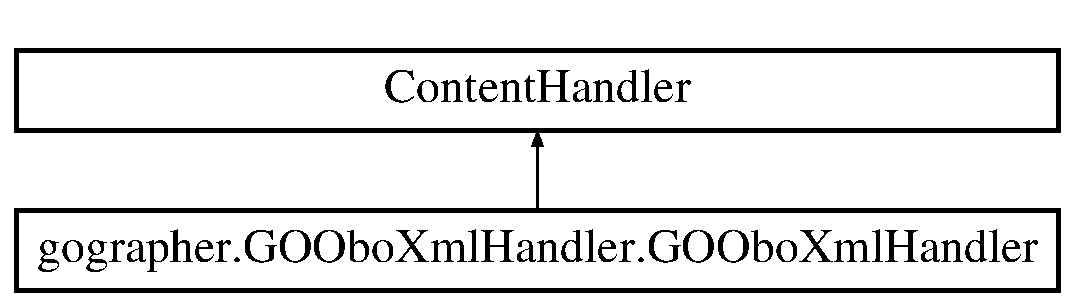
\includegraphics[height=2.000000cm]{classgographer_1_1_g_o_obo_xml_handler_1_1_g_o_obo_xml_handler}
\end{center}
\end{figure}
\subsection*{Public Member Functions}
\begin{DoxyCompactItemize}
\item 
def \hyperlink{classgographer_1_1_g_o_obo_xml_handler_1_1_g_o_obo_xml_handler_a607dac4f99309079ba554cbc63e81df0}{\-\_\-\-\_\-init\-\_\-\-\_\-}
\begin{DoxyCompactList}\small\item\em Constructor. \end{DoxyCompactList}\item 
def \hyperlink{classgographer_1_1_g_o_obo_xml_handler_1_1_g_o_obo_xml_handler_ad2748207a1532b858ab2e7f94861f06d}{start\-Element}
\begin{DoxyCompactList}\small\item\em Create a new element. \end{DoxyCompactList}\item 
def \hyperlink{classgographer_1_1_g_o_obo_xml_handler_1_1_g_o_obo_xml_handler_a91ee43134b69f11fcad5d20b162841a8}{end\-Element}
\begin{DoxyCompactList}\small\item\em Modify an element based on input. \end{DoxyCompactList}\item 
def \hyperlink{classgographer_1_1_g_o_obo_xml_handler_1_1_g_o_obo_xml_handler_a5f2925a757bb5bf9f07696cb8042c2f2}{characters}
\begin{DoxyCompactList}\small\item\em Append additional data. \end{DoxyCompactList}\end{DoxyCompactItemize}
\subsection*{Public Attributes}
\begin{DoxyCompactItemize}
\item 
\hypertarget{classgographer_1_1_g_o_obo_xml_handler_1_1_g_o_obo_xml_handler_a8877634cffd585b24a24ed277531ac7e}{{\bfseries namespace}}\label{classgographer_1_1_g_o_obo_xml_handler_1_1_g_o_obo_xml_handler_a8877634cffd585b24a24ed277531ac7e}

\item 
\hypertarget{classgographer_1_1_g_o_obo_xml_handler_1_1_g_o_obo_xml_handler_abc14c853e0895500d4f9bf0032636428}{{\bfseries graph}}\label{classgographer_1_1_g_o_obo_xml_handler_1_1_g_o_obo_xml_handler_abc14c853e0895500d4f9bf0032636428}

\item 
\hypertarget{classgographer_1_1_g_o_obo_xml_handler_1_1_g_o_obo_xml_handler_a24227cb95fd88b21411500ab0e9f46d1}{{\bfseries in\-Typedef}}\label{classgographer_1_1_g_o_obo_xml_handler_1_1_g_o_obo_xml_handler_a24227cb95fd88b21411500ab0e9f46d1}

\item 
\hypertarget{classgographer_1_1_g_o_obo_xml_handler_1_1_g_o_obo_xml_handler_a4c68b79efd60a75e962aeb3c512eddac}{{\bfseries go\-Node}}\label{classgographer_1_1_g_o_obo_xml_handler_1_1_g_o_obo_xml_handler_a4c68b79efd60a75e962aeb3c512eddac}

\item 
\hypertarget{classgographer_1_1_g_o_obo_xml_handler_1_1_g_o_obo_xml_handler_a43006649fa313bc99bae42fe1fbebfe1}{{\bfseries obsolete}}\label{classgographer_1_1_g_o_obo_xml_handler_1_1_g_o_obo_xml_handler_a43006649fa313bc99bae42fe1fbebfe1}

\item 
\hypertarget{classgographer_1_1_g_o_obo_xml_handler_1_1_g_o_obo_xml_handler_a6652b4cf4642706cd5ea21075bc910a4}{{\bfseries cdata}}\label{classgographer_1_1_g_o_obo_xml_handler_1_1_g_o_obo_xml_handler_a6652b4cf4642706cd5ea21075bc910a4}

\item 
\hypertarget{classgographer_1_1_g_o_obo_xml_handler_1_1_g_o_obo_xml_handler_ac4edc3d1865ee984c47f1afd90c6db4c}{{\bfseries goid}}\label{classgographer_1_1_g_o_obo_xml_handler_1_1_g_o_obo_xml_handler_ac4edc3d1865ee984c47f1afd90c6db4c}

\item 
\hypertarget{classgographer_1_1_g_o_obo_xml_handler_1_1_g_o_obo_xml_handler_aaf4e4a5bac6e9fb07c605497fc447867}{{\bfseries name}}\label{classgographer_1_1_g_o_obo_xml_handler_1_1_g_o_obo_xml_handler_aaf4e4a5bac6e9fb07c605497fc447867}

\item 
\hypertarget{classgographer_1_1_g_o_obo_xml_handler_1_1_g_o_obo_xml_handler_a53835f11cef97190c3e64c6ea8317ff8}{{\bfseries description}}\label{classgographer_1_1_g_o_obo_xml_handler_1_1_g_o_obo_xml_handler_a53835f11cef97190c3e64c6ea8317ff8}

\item 
\hypertarget{classgographer_1_1_g_o_obo_xml_handler_1_1_g_o_obo_xml_handler_a5ca4da66b256fbf8a51107c06bc206c4}{{\bfseries element\-Namespace}}\label{classgographer_1_1_g_o_obo_xml_handler_1_1_g_o_obo_xml_handler_a5ca4da66b256fbf8a51107c06bc206c4}

\item 
\hypertarget{classgographer_1_1_g_o_obo_xml_handler_1_1_g_o_obo_xml_handler_abfc467f1c168119c69183d801c1309db}{{\bfseries parents}}\label{classgographer_1_1_g_o_obo_xml_handler_1_1_g_o_obo_xml_handler_abfc467f1c168119c69183d801c1309db}

\end{DoxyCompactItemize}


\subsection{Detailed Description}
\begin{DoxyVerb}This class handles parsing the OBO XML file from the Gene Ontology Consortium and populate
    a GOGraph object passed to the constructor of this class.  The handler only use the nodes from
    the namespace (a branch of the GO) specificed in the GOGraph object.  Currently, only the edges
    that reflect IS_A relationship between a pair of GO terms are parsed and added into the GOGraph
\end{DoxyVerb}
 

\subsection{Constructor \& Destructor Documentation}
\hypertarget{classgographer_1_1_g_o_obo_xml_handler_1_1_g_o_obo_xml_handler_a607dac4f99309079ba554cbc63e81df0}{\index{gographer\-::\-G\-O\-Obo\-Xml\-Handler\-::\-G\-O\-Obo\-Xml\-Handler@{gographer\-::\-G\-O\-Obo\-Xml\-Handler\-::\-G\-O\-Obo\-Xml\-Handler}!\-\_\-\-\_\-init\-\_\-\-\_\-@{\-\_\-\-\_\-init\-\_\-\-\_\-}}
\index{\-\_\-\-\_\-init\-\_\-\-\_\-@{\-\_\-\-\_\-init\-\_\-\-\_\-}!gographer::GOOboXmlHandler::GOOboXmlHandler@{gographer\-::\-G\-O\-Obo\-Xml\-Handler\-::\-G\-O\-Obo\-Xml\-Handler}}
\subsubsection[{\-\_\-\-\_\-init\-\_\-\-\_\-}]{\setlength{\rightskip}{0pt plus 5cm}def gographer.\-G\-O\-Obo\-Xml\-Handler.\-G\-O\-Obo\-Xml\-Handler.\-\_\-\-\_\-init\-\_\-\-\_\- (
\begin{DoxyParamCaption}
\item[{}]{self, }
\item[{}]{go\-Graph}
\end{DoxyParamCaption}
)}}\label{classgographer_1_1_g_o_obo_xml_handler_1_1_g_o_obo_xml_handler_a607dac4f99309079ba554cbc63e81df0}


Constructor. 


\begin{DoxyParams}{Parameters}
{\em go\-Graph} & A reference to a G\-O\-Graph object to which the parsed G\-O nodes and edges will be added. \\
\hline
\end{DoxyParams}


\subsection{Member Function Documentation}
\hypertarget{classgographer_1_1_g_o_obo_xml_handler_1_1_g_o_obo_xml_handler_a5f2925a757bb5bf9f07696cb8042c2f2}{\index{gographer\-::\-G\-O\-Obo\-Xml\-Handler\-::\-G\-O\-Obo\-Xml\-Handler@{gographer\-::\-G\-O\-Obo\-Xml\-Handler\-::\-G\-O\-Obo\-Xml\-Handler}!characters@{characters}}
\index{characters@{characters}!gographer::GOOboXmlHandler::GOOboXmlHandler@{gographer\-::\-G\-O\-Obo\-Xml\-Handler\-::\-G\-O\-Obo\-Xml\-Handler}}
\subsubsection[{characters}]{\setlength{\rightskip}{0pt plus 5cm}def gographer.\-G\-O\-Obo\-Xml\-Handler.\-G\-O\-Obo\-Xml\-Handler.\-characters (
\begin{DoxyParamCaption}
\item[{}]{self, }
\item[{}]{data}
\end{DoxyParamCaption}
)}}\label{classgographer_1_1_g_o_obo_xml_handler_1_1_g_o_obo_xml_handler_a5f2925a757bb5bf9f07696cb8042c2f2}


Append additional data. 


\begin{DoxyParams}{Parameters}
{\em data} & Additional data to be appended \\
\hline
\end{DoxyParams}
\hypertarget{classgographer_1_1_g_o_obo_xml_handler_1_1_g_o_obo_xml_handler_a91ee43134b69f11fcad5d20b162841a8}{\index{gographer\-::\-G\-O\-Obo\-Xml\-Handler\-::\-G\-O\-Obo\-Xml\-Handler@{gographer\-::\-G\-O\-Obo\-Xml\-Handler\-::\-G\-O\-Obo\-Xml\-Handler}!end\-Element@{end\-Element}}
\index{end\-Element@{end\-Element}!gographer::GOOboXmlHandler::GOOboXmlHandler@{gographer\-::\-G\-O\-Obo\-Xml\-Handler\-::\-G\-O\-Obo\-Xml\-Handler}}
\subsubsection[{end\-Element}]{\setlength{\rightskip}{0pt plus 5cm}def gographer.\-G\-O\-Obo\-Xml\-Handler.\-G\-O\-Obo\-Xml\-Handler.\-end\-Element (
\begin{DoxyParamCaption}
\item[{}]{self, }
\item[{}]{name}
\end{DoxyParamCaption}
)}}\label{classgographer_1_1_g_o_obo_xml_handler_1_1_g_o_obo_xml_handler_a91ee43134b69f11fcad5d20b162841a8}


Modify an element based on input. 


\begin{DoxyParams}{Parameters}
{\em name} & A string set to \char`\"{}id\char`\"{}, \char`\"{}namespace\char`\"{}, \char`\"{}is\-\_\-a\char`\"{}, \char`\"{}is\-\_\-obsolete\char`\"{}, \char`\"{}typedef\char`\"{}, \char`\"{}term\char`\"{}, \char`\"{}name\char`\"{}, or \char`\"{}defstr\char`\"{} depending on the desired changes \\
\hline
\end{DoxyParams}
\hypertarget{classgographer_1_1_g_o_obo_xml_handler_1_1_g_o_obo_xml_handler_ad2748207a1532b858ab2e7f94861f06d}{\index{gographer\-::\-G\-O\-Obo\-Xml\-Handler\-::\-G\-O\-Obo\-Xml\-Handler@{gographer\-::\-G\-O\-Obo\-Xml\-Handler\-::\-G\-O\-Obo\-Xml\-Handler}!start\-Element@{start\-Element}}
\index{start\-Element@{start\-Element}!gographer::GOOboXmlHandler::GOOboXmlHandler@{gographer\-::\-G\-O\-Obo\-Xml\-Handler\-::\-G\-O\-Obo\-Xml\-Handler}}
\subsubsection[{start\-Element}]{\setlength{\rightskip}{0pt plus 5cm}def gographer.\-G\-O\-Obo\-Xml\-Handler.\-G\-O\-Obo\-Xml\-Handler.\-start\-Element (
\begin{DoxyParamCaption}
\item[{}]{self, }
\item[{}]{name, }
\item[{}]{attributes}
\end{DoxyParamCaption}
)}}\label{classgographer_1_1_g_o_obo_xml_handler_1_1_g_o_obo_xml_handler_ad2748207a1532b858ab2e7f94861f06d}


Create a new element. 


\begin{DoxyParams}{Parameters}
{\em name} & Set to either \char`\"{}term\char`\"{} if a new node is to be created or \char`\"{}typedef\char`\"{} if declaring a typedef is desired \\
\hline
{\em attributes} & \\
\hline
\end{DoxyParams}


The documentation for this class was generated from the following file\-:\begin{DoxyCompactItemize}
\item 
/\-Users/\-Zack/\-Desktop/\-Comp\-Sci/cs1680/gographer/G\-O\-Obo\-Xml\-Handler.\-py\end{DoxyCompactItemize}

\hypertarget{classgographer_1_1_g_o_pubmed_graph_1_1_g_o_pubmed_graph}{\section{gographer.\-G\-O\-Pubmed\-Graph.\-G\-O\-Pubmed\-Graph Class Reference}
\label{classgographer_1_1_g_o_pubmed_graph_1_1_g_o_pubmed_graph}\index{gographer.\-G\-O\-Pubmed\-Graph.\-G\-O\-Pubmed\-Graph@{gographer.\-G\-O\-Pubmed\-Graph.\-G\-O\-Pubmed\-Graph}}
}
Inheritance diagram for gographer.\-G\-O\-Pubmed\-Graph.\-G\-O\-Pubmed\-Graph\-:\begin{figure}[H]
\begin{center}
\leavevmode
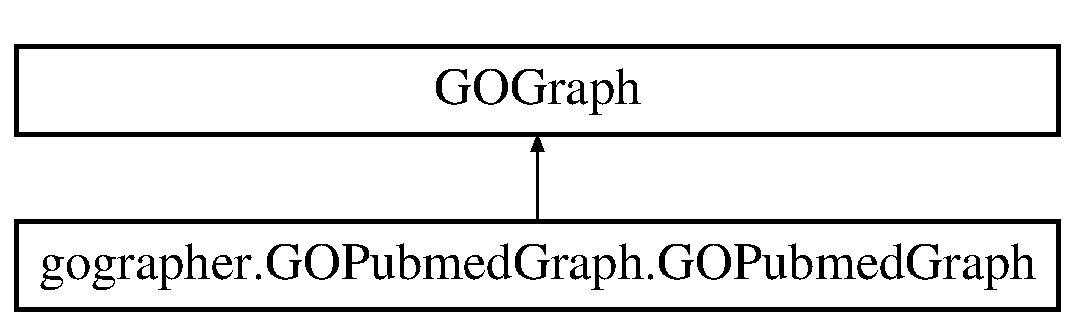
\includegraphics[height=2.000000cm]{classgographer_1_1_g_o_pubmed_graph_1_1_g_o_pubmed_graph}
\end{center}
\end{figure}
\subsection*{Public Member Functions}
\begin{DoxyCompactItemize}
\item 
def \hyperlink{classgographer_1_1_g_o_pubmed_graph_1_1_g_o_pubmed_graph_a189fe767deaf77d733fa53e47163d81a}{\-\_\-\-\_\-init\-\_\-\-\_\-}
\begin{DoxyCompactList}\small\item\em Create a pubmed graph from a G\-O\-Graph. \end{DoxyCompactList}\item 
def \hyperlink{classgographer_1_1_g_o_pubmed_graph_1_1_g_o_pubmed_graph_a3a1f46901b29f0aac04b185f620f24a5}{parse\-Assoc\-File}
\begin{DoxyCompactList}\small\item\em Parses the given association file and adds the pubmed information to the appropriate nodes. \end{DoxyCompactList}\item 
\hypertarget{classgographer_1_1_g_o_pubmed_graph_1_1_g_o_pubmed_graph_ad09c08e73d20d8cd50dddd1b8d9c1e19}{def \hyperlink{classgographer_1_1_g_o_pubmed_graph_1_1_g_o_pubmed_graph_ad09c08e73d20d8cd50dddd1b8d9c1e19}{weight}}\label{classgographer_1_1_g_o_pubmed_graph_1_1_g_o_pubmed_graph_ad09c08e73d20d8cd50dddd1b8d9c1e19}

\begin{DoxyCompactList}\small\item\em Applies a weight to the graph. \end{DoxyCompactList}\item 
def \hyperlink{classgographer_1_1_g_o_pubmed_graph_1_1_g_o_pubmed_graph_a1c154dbc02edbf83254ee5cb5b20fb44}{to\-G\-O\-Gene\-Pubmed\-Graph}
\begin{DoxyCompactList}\small\item\em Returns a G\-O\-Gene\-Pubmed\-Graph version of itself. \end{DoxyCompactList}\item 
def \hyperlink{classgographer_1_1_g_o_pubmed_graph_1_1_g_o_pubmed_graph_a29482c641bfcdf4c98a6d9040f4f5f48}{get\-Pub\-Med\-By\-Node}
\begin{DoxyCompactList}\small\item\em Returns the associated Pub\-Med I\-Ds for a given node. \end{DoxyCompactList}\item 
def \hyperlink{classgographer_1_1_g_o_pubmed_graph_1_1_g_o_pubmed_graph_a983edce6ae320ee5cf42a6a7dee4695f}{get\-Propagated\-Pub\-Med\-By\-Node}
\begin{DoxyCompactList}\small\item\em Returns the associated propagated Pub\-Med I\-Ds for a given node. \end{DoxyCompactList}\item 
def \hyperlink{classgographer_1_1_g_o_pubmed_graph_1_1_g_o_pubmed_graph_a13c9486adf5d33fb73d52f4ed6eb847d}{get\-Nodes\-By\-Pub\-Med}
\begin{DoxyCompactList}\small\item\em Returns the associated nodes for a given Pub\-Med I\-D. \end{DoxyCompactList}\item 
\hypertarget{classgographer_1_1_g_o_pubmed_graph_1_1_g_o_pubmed_graph_affafb8539de441b7a6657923a5d5ba2a}{def \hyperlink{classgographer_1_1_g_o_pubmed_graph_1_1_g_o_pubmed_graph_affafb8539de441b7a6657923a5d5ba2a}{propagate\-P\-M\-I\-Ds}}\label{classgographer_1_1_g_o_pubmed_graph_1_1_g_o_pubmed_graph_affafb8539de441b7a6657923a5d5ba2a}

\begin{DoxyCompactList}\small\item\em Propagate the P\-M\-I\-Ds associated with each node to its parents. \end{DoxyCompactList}\item 
def \hyperlink{classgographer_1_1_g_o_pubmed_graph_1_1_g_o_pubmed_graph_aebb4c16c82e92debadf145153f0c519a}{calculate\-Word\-Vectors}
\begin{DoxyCompactList}\small\item\em Calculates the word vectors for all of the nodes in the graph. \end{DoxyCompactList}\item 
\hypertarget{classgographer_1_1_g_o_pubmed_graph_1_1_g_o_pubmed_graph_afec207ccd7c52eecce6d972aa4398ba0}{def \hyperlink{classgographer_1_1_g_o_pubmed_graph_1_1_g_o_pubmed_graph_afec207ccd7c52eecce6d972aa4398ba0}{remove\-P\-M\-I\-Dless}}\label{classgographer_1_1_g_o_pubmed_graph_1_1_g_o_pubmed_graph_afec207ccd7c52eecce6d972aa4398ba0}

\begin{DoxyCompactList}\small\item\em Remove nodes that don't have at least one associated P\-M\-I\-D. \end{DoxyCompactList}\end{DoxyCompactItemize}
\subsection*{Public Attributes}
\begin{DoxyCompactItemize}
\item 
\hypertarget{classgographer_1_1_g_o_pubmed_graph_1_1_g_o_pubmed_graph_a6dde52b3e51a9c0cfb42c9748cc97594}{{\bfseries pubmed\-To\-Node}}\label{classgographer_1_1_g_o_pubmed_graph_1_1_g_o_pubmed_graph_a6dde52b3e51a9c0cfb42c9748cc97594}

\item 
\hypertarget{classgographer_1_1_g_o_pubmed_graph_1_1_g_o_pubmed_graph_aa537adde73c93b4e611bb2b2f4a7d17b}{{\bfseries exclude\-Evidence}}\label{classgographer_1_1_g_o_pubmed_graph_1_1_g_o_pubmed_graph_aa537adde73c93b4e611bb2b2f4a7d17b}

\end{DoxyCompactItemize}


\subsection{Constructor \& Destructor Documentation}
\hypertarget{classgographer_1_1_g_o_pubmed_graph_1_1_g_o_pubmed_graph_a189fe767deaf77d733fa53e47163d81a}{\index{gographer\-::\-G\-O\-Pubmed\-Graph\-::\-G\-O\-Pubmed\-Graph@{gographer\-::\-G\-O\-Pubmed\-Graph\-::\-G\-O\-Pubmed\-Graph}!\-\_\-\-\_\-init\-\_\-\-\_\-@{\-\_\-\-\_\-init\-\_\-\-\_\-}}
\index{\-\_\-\-\_\-init\-\_\-\-\_\-@{\-\_\-\-\_\-init\-\_\-\-\_\-}!gographer::GOPubmedGraph::GOPubmedGraph@{gographer\-::\-G\-O\-Pubmed\-Graph\-::\-G\-O\-Pubmed\-Graph}}
\subsubsection[{\-\_\-\-\_\-init\-\_\-\-\_\-}]{\setlength{\rightskip}{0pt plus 5cm}def gographer.\-G\-O\-Pubmed\-Graph.\-G\-O\-Pubmed\-Graph.\-\_\-\-\_\-init\-\_\-\-\_\- (
\begin{DoxyParamCaption}
\item[{}]{self, }
\item[{}]{gograph, }
\item[{}]{assoc = {\ttfamily None}, }
\item[{}]{exclude\-Evidence = {\ttfamily \mbox{[}\mbox{]}}, }
\item[{}]{types = {\ttfamily \mbox{[}\char`\"{}protein\char`\"{}\mbox{]}}}
\end{DoxyParamCaption}
)}}\label{classgographer_1_1_g_o_pubmed_graph_1_1_g_o_pubmed_graph_a189fe767deaf77d733fa53e47163d81a}


Create a pubmed graph from a G\-O\-Graph. 


\begin{DoxyParams}{Parameters}
{\em gograph} & A G\-O\-Graph to base this graph off of \\
\hline
{\em assoc} & The file containing gene and pubmed association information \\
\hline
{\em exclude\-Evidence} & A list of the evidence codes that should be ignored \\
\hline
\end{DoxyParams}


\subsection{Member Function Documentation}
\hypertarget{classgographer_1_1_g_o_pubmed_graph_1_1_g_o_pubmed_graph_aebb4c16c82e92debadf145153f0c519a}{\index{gographer\-::\-G\-O\-Pubmed\-Graph\-::\-G\-O\-Pubmed\-Graph@{gographer\-::\-G\-O\-Pubmed\-Graph\-::\-G\-O\-Pubmed\-Graph}!calculate\-Word\-Vectors@{calculate\-Word\-Vectors}}
\index{calculate\-Word\-Vectors@{calculate\-Word\-Vectors}!gographer::GOPubmedGraph::GOPubmedGraph@{gographer\-::\-G\-O\-Pubmed\-Graph\-::\-G\-O\-Pubmed\-Graph}}
\subsubsection[{calculate\-Word\-Vectors}]{\setlength{\rightskip}{0pt plus 5cm}def gographer.\-G\-O\-Pubmed\-Graph.\-G\-O\-Pubmed\-Graph.\-calculate\-Word\-Vectors (
\begin{DoxyParamCaption}
\item[{}]{self, }
\item[{}]{corpus, }
\item[{}]{tokenizer = {\ttfamily {\bf Tokenizer}().tokenize\-\_\-word}, }
\item[{}]{stemmer = {\ttfamily {\bf Porter\-Stemmer}().stem}, }
\item[{}]{stopwords = {\ttfamily \mbox{[}\mbox{]}}}
\end{DoxyParamCaption}
)}}\label{classgographer_1_1_g_o_pubmed_graph_1_1_g_o_pubmed_graph_aebb4c16c82e92debadf145153f0c519a}


Calculates the word vectors for all of the nodes in the graph. 


\begin{DoxyParams}{Parameters}
{\em corpus} & The corpus that contains the information on the Pub\-Med article \\
\hline
{\em tokenizer} & The tokenizer function that will be used on the text, a simple tokenizer is used if none is given. Should take a string as an input, and outputs a string with words that are lower case and separated by a space \\
\hline
{\em stemmer} & The stemmer function that will be used to stem the words, the porter stemmer is used if none is given Takes a word as an input and reports a stemmed word as an output. \\
\hline
{\em stopwords} & A list of stop words that will not be included in the word vector, either as a list or a Stopword\-List. An empty list is used if no stop word list is given. \\
\hline
\end{DoxyParams}
\hypertarget{classgographer_1_1_g_o_pubmed_graph_1_1_g_o_pubmed_graph_a13c9486adf5d33fb73d52f4ed6eb847d}{\index{gographer\-::\-G\-O\-Pubmed\-Graph\-::\-G\-O\-Pubmed\-Graph@{gographer\-::\-G\-O\-Pubmed\-Graph\-::\-G\-O\-Pubmed\-Graph}!get\-Nodes\-By\-Pub\-Med@{get\-Nodes\-By\-Pub\-Med}}
\index{get\-Nodes\-By\-Pub\-Med@{get\-Nodes\-By\-Pub\-Med}!gographer::GOPubmedGraph::GOPubmedGraph@{gographer\-::\-G\-O\-Pubmed\-Graph\-::\-G\-O\-Pubmed\-Graph}}
\subsubsection[{get\-Nodes\-By\-Pub\-Med}]{\setlength{\rightskip}{0pt plus 5cm}def gographer.\-G\-O\-Pubmed\-Graph.\-G\-O\-Pubmed\-Graph.\-get\-Nodes\-By\-Pub\-Med (
\begin{DoxyParamCaption}
\item[{}]{self, }
\item[{}]{pubmed}
\end{DoxyParamCaption}
)}}\label{classgographer_1_1_g_o_pubmed_graph_1_1_g_o_pubmed_graph_a13c9486adf5d33fb73d52f4ed6eb847d}


Returns the associated nodes for a given Pub\-Med I\-D. 


\begin{DoxyParams}{Parameters}
{\em pubmed} & The Pub\-Med I\-D for which to retrieve the associated nodes\-: \\
\hline
\end{DoxyParams}
\hypertarget{classgographer_1_1_g_o_pubmed_graph_1_1_g_o_pubmed_graph_a983edce6ae320ee5cf42a6a7dee4695f}{\index{gographer\-::\-G\-O\-Pubmed\-Graph\-::\-G\-O\-Pubmed\-Graph@{gographer\-::\-G\-O\-Pubmed\-Graph\-::\-G\-O\-Pubmed\-Graph}!get\-Propagated\-Pub\-Med\-By\-Node@{get\-Propagated\-Pub\-Med\-By\-Node}}
\index{get\-Propagated\-Pub\-Med\-By\-Node@{get\-Propagated\-Pub\-Med\-By\-Node}!gographer::GOPubmedGraph::GOPubmedGraph@{gographer\-::\-G\-O\-Pubmed\-Graph\-::\-G\-O\-Pubmed\-Graph}}
\subsubsection[{get\-Propagated\-Pub\-Med\-By\-Node}]{\setlength{\rightskip}{0pt plus 5cm}def gographer.\-G\-O\-Pubmed\-Graph.\-G\-O\-Pubmed\-Graph.\-get\-Propagated\-Pub\-Med\-By\-Node (
\begin{DoxyParamCaption}
\item[{}]{self, }
\item[{}]{goid}
\end{DoxyParamCaption}
)}}\label{classgographer_1_1_g_o_pubmed_graph_1_1_g_o_pubmed_graph_a983edce6ae320ee5cf42a6a7dee4695f}


Returns the associated propagated Pub\-Med I\-Ds for a given node. 


\begin{DoxyParams}{Parameters}
{\em goid} & The G\-O\-I\-D of the node to retrieve the associated propagated Pub\-Med I\-Ds from \\
\hline
\end{DoxyParams}
\hypertarget{classgographer_1_1_g_o_pubmed_graph_1_1_g_o_pubmed_graph_a29482c641bfcdf4c98a6d9040f4f5f48}{\index{gographer\-::\-G\-O\-Pubmed\-Graph\-::\-G\-O\-Pubmed\-Graph@{gographer\-::\-G\-O\-Pubmed\-Graph\-::\-G\-O\-Pubmed\-Graph}!get\-Pub\-Med\-By\-Node@{get\-Pub\-Med\-By\-Node}}
\index{get\-Pub\-Med\-By\-Node@{get\-Pub\-Med\-By\-Node}!gographer::GOPubmedGraph::GOPubmedGraph@{gographer\-::\-G\-O\-Pubmed\-Graph\-::\-G\-O\-Pubmed\-Graph}}
\subsubsection[{get\-Pub\-Med\-By\-Node}]{\setlength{\rightskip}{0pt plus 5cm}def gographer.\-G\-O\-Pubmed\-Graph.\-G\-O\-Pubmed\-Graph.\-get\-Pub\-Med\-By\-Node (
\begin{DoxyParamCaption}
\item[{}]{self, }
\item[{}]{goid}
\end{DoxyParamCaption}
)}}\label{classgographer_1_1_g_o_pubmed_graph_1_1_g_o_pubmed_graph_a29482c641bfcdf4c98a6d9040f4f5f48}


Returns the associated Pub\-Med I\-Ds for a given node. 


\begin{DoxyParams}{Parameters}
{\em goid} & The G\-O\-I\-D of the node to retrieve the associated Pub\-Med I\-Ds from \\
\hline
\end{DoxyParams}
\hypertarget{classgographer_1_1_g_o_pubmed_graph_1_1_g_o_pubmed_graph_a3a1f46901b29f0aac04b185f620f24a5}{\index{gographer\-::\-G\-O\-Pubmed\-Graph\-::\-G\-O\-Pubmed\-Graph@{gographer\-::\-G\-O\-Pubmed\-Graph\-::\-G\-O\-Pubmed\-Graph}!parse\-Assoc\-File@{parse\-Assoc\-File}}
\index{parse\-Assoc\-File@{parse\-Assoc\-File}!gographer::GOPubmedGraph::GOPubmedGraph@{gographer\-::\-G\-O\-Pubmed\-Graph\-::\-G\-O\-Pubmed\-Graph}}
\subsubsection[{parse\-Assoc\-File}]{\setlength{\rightskip}{0pt plus 5cm}def gographer.\-G\-O\-Pubmed\-Graph.\-G\-O\-Pubmed\-Graph.\-parse\-Assoc\-File (
\begin{DoxyParamCaption}
\item[{}]{self, }
\item[{}]{assoc, }
\item[{}]{types = {\ttfamily \mbox{[}\char`\"{}protein\char`\"{}\mbox{]}}}
\end{DoxyParamCaption}
)}}\label{classgographer_1_1_g_o_pubmed_graph_1_1_g_o_pubmed_graph_a3a1f46901b29f0aac04b185f620f24a5}


Parses the given association file and adds the pubmed information to the appropriate nodes. 


\begin{DoxyParams}{Parameters}
{\em assoc} & The name of the association file to be parsed \\
\hline
\end{DoxyParams}
\hypertarget{classgographer_1_1_g_o_pubmed_graph_1_1_g_o_pubmed_graph_a1c154dbc02edbf83254ee5cb5b20fb44}{\index{gographer\-::\-G\-O\-Pubmed\-Graph\-::\-G\-O\-Pubmed\-Graph@{gographer\-::\-G\-O\-Pubmed\-Graph\-::\-G\-O\-Pubmed\-Graph}!to\-G\-O\-Gene\-Pubmed\-Graph@{to\-G\-O\-Gene\-Pubmed\-Graph}}
\index{to\-G\-O\-Gene\-Pubmed\-Graph@{to\-G\-O\-Gene\-Pubmed\-Graph}!gographer::GOPubmedGraph::GOPubmedGraph@{gographer\-::\-G\-O\-Pubmed\-Graph\-::\-G\-O\-Pubmed\-Graph}}
\subsubsection[{to\-G\-O\-Gene\-Pubmed\-Graph}]{\setlength{\rightskip}{0pt plus 5cm}def gographer.\-G\-O\-Pubmed\-Graph.\-G\-O\-Pubmed\-Graph.\-to\-G\-O\-Gene\-Pubmed\-Graph (
\begin{DoxyParamCaption}
\item[{}]{self}
\end{DoxyParamCaption}
)}}\label{classgographer_1_1_g_o_pubmed_graph_1_1_g_o_pubmed_graph_a1c154dbc02edbf83254ee5cb5b20fb44}


Returns a G\-O\-Gene\-Pubmed\-Graph version of itself. 


\begin{DoxyParams}{Parameters}
{\em gogenegraph} & The G\-O\-Gene\-Graph that this graph is to be merged with \\
\hline
\end{DoxyParams}


The documentation for this class was generated from the following file\-:\begin{DoxyCompactItemize}
\item 
/\-Users/\-Zack/\-Desktop/\-Comp\-Sci/cs1680/gographer/G\-O\-Pubmed\-Graph.\-py\end{DoxyCompactItemize}

\input{classgographer_1_1_porter_stemmer_1_1_porter_stemmer}
\input{classgographer_1_1_tokenizer_1_1_tokenizer}
\chapter{File Documentation}
\input{____init_____8py}
\input{_corpus_8py}
\input{_document_8py}
\hypertarget{_g_o_gene_graph_8py}{
\section{/Users/vickychen/Documents/Projects/myGOGrapher/gographer/GOGeneGraph.py File Reference}
\label{_g_o_gene_graph_8py}\index{/Users/vickychen/Documents/Projects/myGOGrapher/gographer/GOGeneGraph.py@{/Users/vickychen/Documents/Projects/myGOGrapher/gographer/GOGeneGraph.py}}
}
\subsection*{Classes}
\begin{DoxyCompactItemize}
\item 
class \hyperlink{classgographer_1_1_g_o_gene_graph_1_1_g_o_gene_graph}{gographer.GOGeneGraph.GOGeneGraph}
\end{DoxyCompactItemize}
\subsection*{Packages}
\begin{DoxyCompactItemize}
\item 
package \hyperlink{namespacegographer_1_1_g_o_gene_graph}{gographer.GOGeneGraph}
\item 
package \hyperlink{namespace_g_o_gene_graph}{GOGeneGraph}
\end{DoxyCompactItemize}

\hypertarget{_g_o_gene_pubmed_graph_8py}{
\section{/Users/vickychen/Documents/Projects/myGOGrapher/gographer/GOGenePubmedGraph.py File Reference}
\label{_g_o_gene_pubmed_graph_8py}\index{/Users/vickychen/Documents/Projects/myGOGrapher/gographer/GOGenePubmedGraph.py@{/Users/vickychen/Documents/Projects/myGOGrapher/gographer/GOGenePubmedGraph.py}}
}
\subsection*{Classes}
\begin{DoxyCompactItemize}
\item 
class \hyperlink{class_g_o_gene_pubmed_graph_1_1_g_o_gene_pubmed_graph}{GOGenePubmedGraph.GOGenePubmedGraph}
\end{DoxyCompactItemize}
\subsection*{Packages}
\begin{DoxyCompactItemize}
\item 
package \hyperlink{namespace_g_o_gene_pubmed_graph}{GOGenePubmedGraph}
\end{DoxyCompactItemize}

\hypertarget{_g_o_graph_8py}{
\section{/Users/vickychen/Documents/Projects/myGOGrapher/gographer/GOGraph.py File Reference}
\label{_g_o_graph_8py}\index{/Users/vickychen/Documents/Projects/myGOGrapher/gographer/GOGraph.py@{/Users/vickychen/Documents/Projects/myGOGrapher/gographer/GOGraph.py}}
}
\subsection*{Classes}
\begin{DoxyCompactItemize}
\item 
class \hyperlink{classgographer_1_1_g_o_graph_1_1_g_o_graph}{gographer.GOGraph.GOGraph}
\end{DoxyCompactItemize}
\subsection*{Packages}
\begin{DoxyCompactItemize}
\item 
package \hyperlink{namespacegographer_1_1_g_o_graph}{gographer.GOGraph}
\end{DoxyCompactItemize}

\hypertarget{_g_o_node_8py}{
\section{/Users/vickychen/Documents/Projects/myGOGrapher/gographer/GONode.py File Reference}
\label{_g_o_node_8py}\index{/Users/vickychen/Documents/Projects/myGOGrapher/gographer/GONode.py@{/Users/vickychen/Documents/Projects/myGOGrapher/gographer/GONode.py}}
}
\subsection*{Classes}
\begin{DoxyCompactItemize}
\item 
class \hyperlink{class_g_o_node_1_1_g_o_node}{GONode.GONode}
\end{DoxyCompactItemize}
\subsection*{Packages}
\begin{DoxyCompactItemize}
\item 
package \hyperlink{namespace_g_o_node}{GONode}
\end{DoxyCompactItemize}

\hypertarget{_g_o_obo_xml_handler_8py}{
\section{/Users/vickychen/Documents/Projects/myGOGrapher/gographer/GOOboXmlHandler.py File Reference}
\label{_g_o_obo_xml_handler_8py}\index{/Users/vickychen/Documents/Projects/myGOGrapher/gographer/GOOboXmlHandler.py@{/Users/vickychen/Documents/Projects/myGOGrapher/gographer/GOOboXmlHandler.py}}
}
\subsection*{Classes}
\begin{DoxyCompactItemize}
\item 
class \hyperlink{classgographer_1_1_g_o_obo_xml_handler_1_1_g_o_obo_xml_handler}{gographer.GOOboXmlHandler.GOOboXmlHandler}
\end{DoxyCompactItemize}
\subsection*{Packages}
\begin{DoxyCompactItemize}
\item 
package \hyperlink{namespacegographer_1_1_g_o_obo_xml_handler}{gographer.GOOboXmlHandler}
\end{DoxyCompactItemize}

\hypertarget{_g_o_pubmed_graph_8py}{
\section{/Users/vickychen/Documents/Projects/myGOGrapher/gographer/GOPubmedGraph.py File Reference}
\label{_g_o_pubmed_graph_8py}\index{/Users/vickychen/Documents/Projects/myGOGrapher/gographer/GOPubmedGraph.py@{/Users/vickychen/Documents/Projects/myGOGrapher/gographer/GOPubmedGraph.py}}
}
\subsection*{Classes}
\begin{DoxyCompactItemize}
\item 
class \hyperlink{class_g_o_pubmed_graph_1_1_g_o_pubmed_graph}{GOPubmedGraph.GOPubmedGraph}
\end{DoxyCompactItemize}
\subsection*{Packages}
\begin{DoxyCompactItemize}
\item 
package \hyperlink{namespace_g_o_pubmed_graph}{GOPubmedGraph}
\end{DoxyCompactItemize}

\input{_porter_stemmer_8py}
\hypertarget{test_8py}{
\section{/Users/vickychen/Documents/Projects/myGOGrapher/gographer/test.py File Reference}
\label{test_8py}\index{/Users/vickychen/Documents/Projects/myGOGrapher/gographer/test.py@{/Users/vickychen/Documents/Projects/myGOGrapher/gographer/test.py}}
}
\subsection*{Packages}
\begin{DoxyCompactItemize}
\item 
package \hyperlink{namespacetest}{test}
\end{DoxyCompactItemize}
\subsection*{Variables}
\begin{DoxyCompactItemize}
\item 
string \hyperlink{namespacetest_a4ee7d63d9426ae32ba96ad2f0e171511}{test.location} = \char`\"{}./go\_\-daily-\/termdb.obo-\/xml\char`\"{}
\item 
tuple \hyperlink{namespacetest_a49256f3800de70e9aabf11ea0c3bb8e1}{test.GOGraphtest} = GOGraph(\char`\"{}biological\_\-process\char`\"{}, location)
\item 
string \hyperlink{namespacetest_afe7b4432163ad853f4fcd650d0ecab8c}{test.descrip} = 'The chemical reactions and pathways involving (R)-\/4-\/hydroxymandelate, the anion of a hydroxylated derivative of mandelate (alpha-\/hydroxybenzeneacetate).'
\item 
string \hyperlink{namespacetest_a1429061289985226ca44c2e4e888d77e}{test.namespace} = 'biological\_\-process'
\item 
string \hyperlink{namespacetest_adb8b1e2a5df72522e42bc012571e75cd}{test.assoc} = \char`\"{}./gene\_\-association.goa\_\-human\char`\"{}
\item 
tuple \hyperlink{namespacetest_ab48a47ac8dcf21d32cff24c492f085c1}{test.GOGenetest} = GOGeneGraph(GOGraphtest,assoc)
\item 
tuple \hyperlink{namespacetest_a836657c6fd789469b5cbdd3c88513f7f}{test.genes} = set(\mbox{[}('P05091', ''), ('Q8NE62', ''), ('P47895', ''), ('P48448', ''), ('P00326', ''), ('P43353', ''), ('P08319', ''), ('P07327', '')\mbox{]})
\item 
tuple \hyperlink{namespacetest_a6b190968f9c7fc0593c63df10224e21a}{test.propGenes} = set(\mbox{[}('Q8NE62', ''), ('P47895', ''), ('O43704', ''), ('P48448', ''), ('P43353', ''), ('P05091', ''), ('P00326', ''), ('P08319', ''), ('P07327', '')\mbox{]})
\item 
tuple \hyperlink{namespacetest_aa8cc3a0b86b4a37acf878753845ac845}{test.nodesByGene} = set(\mbox{[}'GO:0006066', 'GO:0008152'\mbox{]})
\item 
tuple \hyperlink{namespacetest_a2565076d50762c7d466830ecbabb1671}{test.GOPubmedtest} = GOPubmedGraph(GOGraphtest,assoc)
\item 
tuple \hyperlink{namespacetest_aa3b15c95748b55bb3ace649b708b6133}{test.pubmed} = set(\mbox{[}('2347582', ''), ('7698756', ''), ('1306115', ''), ('3466164', ''), ('7828891', ''), ('8890755', '')\mbox{]})
\item 
tuple \hyperlink{namespacetest_adc1d0604ecf3fb36f0df45313768ab39}{test.propPubmed} = set(\mbox{[}('10203017', ''), ('7959792', ''), ('9473496', ''), ('7663508', ''), ('10692104', ''), ('6548414', ''), ('3466164', ''), ('10359671', ''), ('11300766', ''), ('11254442', ''), ('9000139', ''), ('10022914', ''), ('8822211', ''), ('10373482', ''), ('1695324', ''), ('1374385', ''), ('3800996', ''), ('12882974', ''), ('3755672', ''), ('9500206', ''), ('8890755', ''), ('8353497', ''), ('9733774', ''), ('9263035', ''), ('8707889', ''), ('9295054', ''), ('7698756', ''), ('8333863', ''), ('7912130', ''), ('9207799', ''), ('11597136', ''), ('9305759', ''), ('2347582', ''), ('10101297', ''), ('8359595', ''), ('11606197', ''), ('1918003', ''), ('1306115', ''), ('9268630', ''), ('9299468', ''), ('10382971', ''), ('9463486', ''), ('11179693', ''), ('9237672', ''), ('7828891', ''), ('9207021', ''), ('2110361', '')\mbox{]})
\end{DoxyCompactItemize}

\input{_tokenizer_8py}
\input{utils_8py}
\printindex
\end{document}
